\documentclass[prd,twocolumn,nofootinbib,superscriptaddress,amsmath,amssymb]{revtex4-1}
\usepackage{mathtools}
\usepackage{graphics}
\usepackage{graphicx}
\graphicspath{{./images/}}
\usepackage{dcolumn}
\usepackage{bm}
\usepackage{dsfont} 
\usepackage{amsmath,amssymb}
\usepackage{hyperref}
\usepackage{tabularx}
%\usepackage{epstopdf}
\usepackage{epsf,epsfig}
\usepackage[normalem]{ulem}
\usepackage[usenames]{color}
\usepackage{multirow}
\usepackage{makecell}
\usepackage{diagbox}
\usepackage[abs]{overpic}
%\epstopdfsetup{outdir=./images/}
\allowdisplaybreaks
\hypersetup{
    colorlinks=true,
    linkcolor=blue,
    filecolor=magenta,      
    urlcolor=blue,
    citecolor=blue
}
\urlstyle{same}


\newcommand{\red}[1]{\protect\color{red} #1 \protect\color{black}}
\newcommand{\green}[1]{\protect\color{green} #1 \protect\color{black}}
\newcommand{\blue}[1]{\protect\color{blue} #1 \protect\color{black}}
\newcommand{\black}[1]{\protect\color{black} #1 \protect\color{black}}
\newcommand{\yellow}[1]{\protect\color{yellow} #1 \protect\color{black}}
\newcommand{\bra}[1]{\protect\langle #1 |}
\newcommand{\ket}[1]{| #1 \protect\rangle}
\newcommand{\braket}[2]{\protect\langle #1 | #2 \protect\rangle}
\newcommand{\expected}[1]{\protect\langle #1 \protect\rangle}
\newcommand{\R}{{\mbox{\tiny R}}}
\newcommand{\ky}[1]{\textcolor{blue}{\it{\textbf{ky: #1}}} }
\newcommand{\kent}[1]{\textcolor{magenta}{\textbf{ #1}} }
\newcommand{\zack}[1]{\textcolor{magenta}{\textbf{ #1}} }
\newcommand{\zc}[1]{\textcolor{red}{\it{\textbf{zc: #1}}} }
\definecolor{red(ncs)}{rgb}{0.77, 0.01, 0.2}
\newcommand{\ny}[1]{\textcolor{blue}{NY: #1} }
\newcommand{\kc}[1]{\textcolor{green}{KC: #1} }
\newcommand{\NS}{{\mbox{\tiny NS}}}
\newcommand{\sci}[2]{#1 \times 10^{#2}}

\usepackage{array}
\newcolumntype{C}[1]{>{\centering\let\newline\\\arraybackslash\hspace{0pt}}m{#1}}


\newcolumntype{C}[1]{>{\centering\arraybackslash}m{#1}}

\def\eq#1{Eq.~(\ref{eq:#1})}
\def\Eq#1{Equation~(\ref{eq:#1})}
\def\eqs#1#2{Eqs.~(\ref{eq:#1}) \& (\ref{eq:#2})}
\def\eqlist#1#2{Eqs.~(\ref{eq:#1}-\ref{eq:#2})}
\def\Eqs#1#2{Equations~(\ref{eq:#1}) \& (\ref{eq:#2})}
\def\Eqlist#1#2{Equations~(\ref{eq:#1}-\ref{eq:#2})}
\def\fig#1{Fig.\ref{fig:#1}}
\def\figs#1#2{Figs.\ref{fig:#1} \& \ref{fig:#2}}
\def\Fig#1{Figure~\ref{fig:#1}}
\def\Figs#1#2{Figures~\ref{fig:#1} \& \ref{fig:#2}}
\def\tab#1{Table~\ref{tab:#1}}
\def\sec#1{Section~\ref{sec:#1}}



\begin{document}

\title{Equation-of-state insensitive relations after GW170817}

\author{Zachary Carson}
\affiliation{%
 Department of Physics, University of Virginia, Charlottesville, Virginia 22904, USA
}%

\author{Katerina Chatziioannou}
%\affiliation{%
% Canadian Institute for Theoretical Astrophysics, 60 St. George Street, Toronto, Ontario, M5S 3H8, Canada
%}%
\affiliation{%
 Center for Computational Astrophysics, Flatiron Institute, 162 5th Ave, New York, NY 10010
}%

\author{Carl-Johan Haster}
\affiliation{%
 Canadian Institute for Theoretical Astrophysics, 60 St. George Street, Toronto, Ontario, M5S 3H8, Canada
}%
\affiliation{%
 Center for Computational Astrophysics, Flatiron Institute, 162 5th Ave, New York, NY 10010
}%

\author{Nicol\'as Yunes}
\affiliation{%
eXtreme Gravity Institute, Department of Physics, Montana State University, Bozeman, MT 59717, USA.
}%
\affiliation{%
 Department of Physics and MIT Kavli Institute,
}%

\author{Kent Yagi}
\affiliation{%
 Department of Physics, University of Virginia, Charlottesville, Virginia 22904, USA
}%


\date{\today}

%%%%%%%%%%%%%%%%%%
%%%%%%%%%%%%%%%%%%
%%%% ABSTRACT %%%%
%%%%%%%%%%%%%%%%%%
%%%%%%%%%%%%%%%%%%

\begin{abstract}
% Intro
The thermodynamic relation between pressure and density (i.e.~the equation of state) of cold supranuclear matter is critical to neutron stars, yet it remains one of the largest uncertainties in nuclear physics. 
% How to probe
The extraction of tidal deformabilities from the gravitational waves emitted in the coalescence of neutron star binaries, such as GW170817, is a promising tool to probe this thermodynamic relation.
% What was done before - Binary Love
Equation-of-state insensitive relations between symmetric and antisymmetric combinations of individual tidal deformabilities, the so-called  ``binary Love relations", have proven important to infer the radius of neutron stars, and thus constrain the equation of state, from such gravitational waves. 
% What was done before - I-Love-Q
A similar set of relations between the moment of inertia, the tidal deformability, the quadrupole moment, and the compactness of neutron stars, the so-called ``I-Love-Q" and ``C-Love" relations, allow for future tests of General Relativity in the extreme gravity regime. 
% What we will do
But even the most insensitive of such relations still presents some degree of equation-of-state variability that could introduce systematic uncertainties in parameter extraction and in model selection. 
%
We here reduce this variability by more than $50\%$ by imposing a prior on the allowed set of equations of state, derived from the posteriors generated from the analysis of GW170817.  
%
The resulting increase in insensitivity reduces systematic uncertainties in the extraction of the tidal deformability from future gravitational wave observations, although statistical uncertainties currently dominate the error budget, and will continue to do so until the era of Voyager-class detectors.  
\end{abstract}

\maketitle

%%%%%%%%%%%%%%%%%%%%%%
%%%%%%%%%%%%%%%%%%%%%%
%%%% INTRODUCTION %%%%
%%%%%%%%%%%%%%%%%%%%%%
%%%%%%%%%%%%%%%%%%%%%%

\section{Introduction}
\label{sec:intro}

%Intro
The thermodynamic relation between pressure and density in cold, supranuclear matter, the so-called equation of state (EoS), remains an unsolved problem in nuclear physics. The EoS is critical to our understanding of neutron stars (NSs) because it determines many NS observables, such as their mass, radius, moment of inertia (I), quadrupole moment (Q) and tidal deformability (or Love number). Unfortunately, terrestrial experiments can only probe the EoS to around nuclear saturation density ($\rho_{\text{sat}} \approx 2.5 \times 10^{14} \text{ g/cm}^3$)~\cite{Li:HeavyIon,Tsang:SymmetryEnergy,Centelles:NeutronSkin,Li:CrossSections,Chen:SymEnergy}. Although some temperature-dependent heavy-ion collision experiments are beginning to probe higher densities~\cite{Danielewicz:2002pu}, astrophysical observations of NSs remain ideal for constraining the EoS of cold and ultra dense, nuclear matter.

%Constraining the EoS
Independent measurements of NS observables can be used to constrain the nuclear EoS. For example, electromagnetic observations of the mass and radius of certain NSs have been used to place confidence limits in the mass-radius plane, and thus constrain the EoS~\cite{guver,ozel-baym-guver,steiner-lattimer-brown,Lattimer2014,Ozel:2016oaf}. These observations, however, may potentially suffer from large systematic errors due to uncertainties in the astrophysical modeling of X-ray bursts. The gravitational waves (GWs) emitted in the coalesce of NS binaries may be a cleaner probe of nuclear physics. During the early inspiral, the orbital separation is large enough that the tidal fields are negligible; but as the orbital separation decreases due to GW emission, tidal forces grow and the NSs respond by developing deformations controlled by their nuclear EoS. These deformations affect the orbital trajectory of the binary, and thus the GWs emitted, encoding in the latter the NS EoS~\cite{hinderer-love,Flanagan2008}.

%reparameterization of the template
The GWs emitted by binary NSs in the late inspiral must then depend on the \emph{tidal deformabilities} $\Lambda_1$ and $\Lambda_2$, which control the linear response of the star's quadrupole deformation to the (electric-type, quadrupole) tidal field of the companion (to leading order in a post-Newtonian expansion~\cite{Blanchet:2013haa})~\cite{Flanagan2008,Vines:2011ud}. These parameters, however, enter the GW Fourier model multiplied by the same function of the GW frequency (at leading post-Newtonian order), making them degenerate, and thus, very difficult to estimate independently with current GW data~\cite{Wade:tidalCorrections}. Instead, one can extract certain combinations of the tidal deformabilities, like a certain mass-weighted tidal deformability $\tilde{\Lambda}$~\cite{Favata:2013rwa,Wade:tidalCorrections}, or one can extract the (mass-independent) coefficients $(\lambda_{0},\lambda_{1},\ldots)$ of a Taylor expansion of the tidal deformabilities about some fiducial mass~\cite{delPozzo:TaylorTidal,Yagi:binLove}. Current detectors are not sensitive enough to accurately measure any of these coefficients, but future detectors will and the information from multiple events could then be combined, since the Taylor expansion coefficient should be common to all events. 

%Universal relations
Lacking enough sensitivity in current GW observations, one is forced to only estimate the mass-weighted tidal deformability, but this prevents the independent extraction of $\Lambda_{1}$ and $\Lambda_{2}$. Yagi and Yunes~\cite{Yagi:binLove} solved this problem by finding ``approximately universal'' or ``EoS-insensitive'' relations between the symmetric and anti-symmetric combinations of the tidal deformabilities $\Lambda_{s,a}=\frac{1}{2}(\Lambda_1 \pm \Lambda_2)$, the so-called ``binary Love relations." These relations can be used to analytically express $\Lambda_{s}$ in terms of $\Lambda_{a}$ (or vice-versa), making the mass-weighted tidal deformability a function of only $\Lambda_{a}$. A measurement of the mass-weighted tidal deformability then implies a measurement of $\Lambda_{a}$, and through the use of the binary Love relations, also a measurement of $\Lambda_{s}$, which then allows for the inference of the individual tidal deformabilities $\Lambda_{1}$ and $\Lambda_{2}$~\cite{Yagi:binLove}. With those at hand, one can further use EoS-insensitive relations between the tidal deformabilities and the compactness, the so-called ``C-Love relations''~\cite{Yagi:ILQ}, to infer the radii of the NSs, and thus, to place two constraints in the mass-radius plane, one for each star in the binary~\cite{Yagi:binLove}. This idea was recently implemented in GW170817, allowing for the first EoS-independent constraints on the mass-radius curve using GW data~\cite{LIGO:posterior}.     

EoS-insensitive relations can in fact be used for more than just measuring the nuclear EoS. For years, the theoretical physics community considered the possibility of using measurements of NS properties, like the mass, the radius and the moment of inertia, to constrain deviations from General Relativity in the strong-field regime. Certain modified theories of gravity, like scalar tensor theories with spontaneous scalarization~\cite{Damour:1996ke}, Einstein-Aether and Horava gravity~\cite{Eling:2007xh,Yagi:2013ava,Yagi:2013qpa}, dynamical Chern-Simons gravity~\cite{Yunes:2009ch}, beyond Horndesky theories~\cite{Sakstein:2016oel}, modify such NS observables, but unfortunately, these modifications are typically degenerate with the nuclear EoS. Yagi and Yunes solved this problem by finding EoS-insensitive relations between the moment of inertia, the tidal deformability (or Love number) and the quadrupole moment, the so-called ``I-Love-Q'' relations~\cite{Yagi:ILQ}. Given a measurement of the Love number for a given NS, for example through GW observations, the I-Love-Q relations can be used to infer the moment of inertia or the quadrupole moment. A second independent measurement of either of these two quantities, for example through binary pulsar observations~\cite{Lattimer:2004nj} or observations with the Neutron star Interior Composition ExploreR (NICER)~\cite{Ozel:2015ykl}, then allows an EoS-insensitive test of General Relativity in the strong field regime~\cite{Yagi:ILQ,Gupta:2017vsl}. 

The implementation of the EoS-insensitive relations in data analysis has to somehow contend with the fact that these relations are in fact not exactly universal, but rather present different (albeit small) levels of EoS variability. In the case of the binary Love and C-Love relations to infer the radii of NSs with GW170817, the problem is solved by marginalizing over the EoS variability~\cite{Katerina:residuals}. Presumably, this same procedure can be applied in the future when carrying out tests of General Relativity with the I-Love-Q relations, using a combination of binary pulsar, NICER and GW data. But this marginalization procedure may not always be as important; as constraints in the mass-radius plane become more stringent with future GW observations, the allowed space of EoSs will shrink, which in turn must naturally decrease the degree of EoS variability in all EoS-insensitive relations. This is the main focus of this paper.  


%%%%%%%%%%%%%%%%%%%%%%%%%%%
%%%%%%%%%%%%%%%%%%%%%%%%%%%
%%%% EXECUTIVE SUMMARY %%%%
%%%%%%%%%%%%%%%%%%%%%%%%%%%
%%%%%%%%%%%%%%%%%%%%%%%%%%%

\subsection{Executive Summary}

%How we improved this
We begin by investigating the increase in EoS insensitivity due to the constraints placed by GW170817 on the allowed space of EoSs. We take the 90\% credible region constructed from the posterior probability distributions on the pressure-density plane~\cite{LIGO:posterior} obtained from GW170817~\cite{TheLIGOScientific:2017qsa} as a prior on the set of EoSs that is compatible with this observation. We then generate two large samples of spectral EoSs~\cite{Lindblom:2018rfr}, one in which this prior is enforced (the ``constrained'' sample) and another in which the prior is not enforced (the ``unconstrained'' sample). We repeat the analysis done by Yagi and Yunes~\cite{Yagi:binLove,Yagi:ILQ} on both sets of EoSs and find that the EoS-insensitive relations present less EoS variability with the constrained set. In particular, the EoS-insensitivity increases by a factor of $\sim 60$\% in the binary Love relations (for stars with mass ratio larger than $0.75$), by a factor of $\sim 70\%$ in the C-Love relations, and by factors of $\sim 50$\% in the I-Love-Q relations (see Table~\ref{tab:maxVar} and Fig.~\ref{fig:ILQ} for more details). 

With this study at hand, we then carry out additional related studies on EoS-insensitive relations that go beyond the work in~\cite{Yagi:binLove,Yagi:ILQ}. First, we investigate the relation between the NS radius and its tidal deformability, the R-Love relations, for both sets of EoSs, because these are critical to place constraints on the radius from a measurement of the Love number.  We use the C-Love relations to construct the R-Love relations and find that the maximum EoS variability drops from $\sim 880 {\rm{km}}$ in the unconstrained case to $\sim 360 {\rm{km}}$ in the constrained case (see Sec.~\ref{sec:clove} for more details). Second, we study the EoS-universality of hybrid stars, which experience strong first-order phase transitions from hadronic to quark matter in the core~\cite{Paschalidis2018}. We find that the I-Love-Q and C-Love relations remain EoS-insensitive for these hybrid stars, although the EoS variability increases slightly (see Sec.~\ref{sec:ilq-hyb} and~\ref{sec:clove-hyb} for more details). However, we also find that the binary Love relations are not EoS-insensitive for a mixed binary with a (massive) hybrid star and a (low-mass) hadronic star, due to the large separation in mass-weighted tidal deformability between the constituent stars (see Sec.~\ref{sec:binary} for more details).

Last for not least, we study the importance of using the improved EoS-insensitive relations in future GW observations. The use of EoS-insensitive relations introduces systematic uncertainties in parameter estimation because of the intrinsic non-zero EoS-variability in these relations, which one must marginalize over. These uncertainties are currently irrelevant because statistical uncertainties in parameter estimation are much larger with current detectors. But as the detector sensitivity is improved, the signal-to-noise ratio and the number of events that will be detected will increase, therefore decreasing the statistical uncertainties below the systematic one due to EoS variability. We carry out a simple Fisher analyses to estimate when the statistical uncertainties become comparable to the systematic uncertainties due to EoS variability and find that this occurs for Voyager-class detectors. 

Figure~\ref{fig:stackedFisher} shows this result in more detail. We here present the (Fisher-estimated) statistical uncertainty in the measurement of $\lambda_{0}$ with various detectors (LIGO O2~\cite{aLIGO}, Advanced LIGO (aLIGO)~\cite{aLIGO}, LIGO A\texttt{+} (A\texttt{+})\cite{Ap_Voyager_CE}, Voyager~\cite{Ap_Voyager_CE}, the Einstein Telescope (ET)~\cite{ET}, and the Cosmic Explorer (CE)~\cite{Ap_Voyager_CE}) for an event identical to GW170817. The x-axis shows the signal-to-noise ratio for a GW170817 event detected with each of these detectors. We also present the combined statistical uncertainty $\sigma^A_N$ after $N$ detections with each of these instruments, with the top and bottom of the region representing the most optimistic and pessimistic expectation for the number of detections expected from the binary NS merger rate (see also Table~\ref{tab:variances}). These statistical uncertainties should be compared to the systematic uncertainty in $\lambda_{0}$ due to EoS-variability improved with the constrained set. Observe that the statistical and the systematic uncertainties cross for Voyager-class detectors.

\begin{figure}
\begin{center} 
\includegraphics[width=\columnwidth]{stackedFisher.eps}
\end{center}
\caption{(Color online) Fisher-estimated statistical uncertainties on the extraction of $\lambda_{0}$ with interferometer (O2, aLIGO, A\texttt{+}, Voyager, CE, ET-D) as a function of the signal-to-noise-ratio expected in each of these instruments, given a single GW170817 detection (circles). The statistical uncertainties with ET are lower than with CE in spite of a lower signal-to-noise ratio because the former is more sensitive above 300 Hz, where tidal effects matter the most (see Sec.~\ref{sec:futureObservations} for further discussion). We also plot the combined statistical uncertainty given $N$ observations consistent with the NS binary merger rate for a 1 year observation (regions), with the top and bottom edges of the regions corresponding to optimistic and pessimistic merger rates. These statistical uncertainties should be compared to the systematic uncertainty on the extraction of $\lambda_{0}$ due to EoS-variability (horizontal dashed line). Observe that the statistical and systematic uncertainties cross for Voyager-class detectors. We confirm this conclusion by repeating the statistical analysis with two different waveform models (PhenomD~\cite{PhenomDI,PhenomDII} plus NRTidal corrections~\cite{Samajdar:NRTidal} and PhenomD~\cite{PhenomDI,PhenomDII} plus 6PN tidal corrections~\cite{Wade:tidalCorrections}).}
\label{fig:stackedFisher}
\end{figure} 

%outline
The remainder of this paper presents the details of the results summarized above and it is organized as follows. 
We begin with complementary background and theory material in Sec.~\ref{sec:theory}.
We continue in Sec.~\ref{sec:universal} by finding new and improved binary Love, I-Love-Q, and C-Love relations, and considering how well hybrid star EoSs agree with the EoS-insensitive relations.
We next examine these improved relations and question whether or not they are useful for future interferometers in Sec.~\ref{sec:observations}.
We conclude in Sec.~\ref{sec:conclusion} by discussing our results and mentioning avenues of future work.
Throughout this paper, we have adopted geometric units of $G=1=c$, unless otherwise stated.

%%%%%%%%%%%%%%%%%%%%%%%%%%%%%%%
%%%%%%%%%%%%%%%%%%%%%%%%%%%%%%%
%%%% BACKGROUND AND THEORY %%%%
%%%%%%%%%%%%%%%%%%%%%%%%%%%%%%%
%%%%%%%%%%%%%%%%%%%%%%%%%%%%%%%

\section{Background and theory}\label{sec:theory}

In this section we review how the EoS can be represented analytically
through a spectral decomposition, and how the observation of GW170817
constrains the space of possible EoSs. We then proceed to discuss 
how one computes the tidal deformabilities and the EoS-insensitive relations. 

\subsection{Spectral representations of NS equations of state}
\label{sec:eos}

The structure of a NS and its tidal interactions in a binary system rely heavily on the underlying state function (or equation of state - EoS) describing the relationship between the pressure ($p$) and energy density ($\epsilon$) of nuclear matter.
Given that all currently proposed EoSs utilize certain approximations~\cite{Oertel:Review,Baym:Review}, one method to study a wide range of physically realizable EoSs is to parameterize them such that any realistic EoS can be represented with a small number of parameters.
Spectral representations~\cite{Lindblom:2010bb,Lindblom:2012zi,Lindblom:2013kra,Lindblom:2018rfr,Abbott:2018exr} parameterize EoSs by performing spectral expansions on the adiabatic index $\Gamma(p)$\footnote{Another way of parameterizing EoSs is through a piecewise polytropic formulation~\cite{Read2009,Lackey:2014fwa,Carney:2018sdv}.}:
\begin{equation}
\Gamma(x) = \exp{\sum_k^{N}\gamma_k x^k},
\end{equation}
where $x \equiv \log{(p/p_0)}$ for a minimum pressure $p_0$.
The equation of state is then determined by an integration of the differential equation:
\begin{equation}
\frac{d \epsilon(p)}{dp}=\frac{\epsilon(p)+p}{p \Gamma(p)}.
\end{equation}
Using this formalism, any valid EoS can be approximated through the choice of $N$ spectral coefficients $\gamma_k$, and we here choose $N=4$, tabulated for several common EoSs in Table 1 of~\cite{Lindblom:2018rfr}.

\begin{figure*}
\begin{center} 
\includegraphics[width=\columnwidth]{EoSs.eps}
\includegraphics[width=\columnwidth]{hybridEoSs.eps}
\end{center}
\caption{(Color Online) Left: Small representative samples of the unconstrained (dotted) and constrained (solid) sets, together with the 90\% marginalized posterior distribution from the observation of GW170817 (cyan shaded region)~\cite{LIGO:posterior}. Observe that the there is significantly less variability in the constrained set of EoSs due to the requirement that they be consistent with the GW170817 observation. Right: EoSs for ACS and ACB hybrid stars, each transitioning from a hadronic branch (corresponding to a pure hadronic-matter NS) into a quark-matter branch (quark-matter inner core surrounded by hadronic matter) at various transition pressures $P_{\text{tr}}$. {\ny{There shouldn't be a title in the figures, no?}}
}
\label{fig:eos}
\end{figure*} 

We here wish to consider EoS-insensitive relations using two sets of EoSs: a ``constrained set'' consistent with the observation of GW170817 and an ``unconstrained set'' that does not impose this prior. In \emph{both} cases, we model the EoS with a $C^{0}$-piecewise function that equals the low-density crust EoS of SLy~\cite{Douchin:2001sv} below half nuclear saturation density $\rho_{\text{stitch}}=1.3 \times 10^{14} \text{ g/cm}^3$~\cite{Read2009}, and equals the spectral decomposition described above outside the crust. For the latter, we restrict the spectral coefficients to the ranges $\gamma_0 \in \lbrack 0.2,2 \rbrack$, $\gamma_1 \in \lbrack -1.6,1.7 \rbrack$, $\gamma_2 \in \lbrack -0.6,0.6 \rbrack$, $\gamma_3 \in \lbrack -0.02,0.02 \rbrack$, and the adiabatic index is further restricted to $\Gamma \in \lbrack 0.6,4.5 \rbrack$~\cite{Lindblom:parameters}. Moreover, we impose the following two restrictions:  (i) causality within 10\%, i.e. that the speed of sound of the fluid be less than the speed of light to 10\%, and (ii) a high maximum mass, i.e.~that the resulting EoS supports NSs with masses at least as high as $1.97 \text{ M}_{\odot}$, consistent with astrophysical observations~\cite{Zhao:massiveNS}. 

The unconstrained set is then defined by drawing random samples in the spectral coefficients (within their allowed prior ranges), and then eliminating any EoS that either leads to a polytropic index $\Gamma$ outside the allowed range, breaks the causality restriction, or breaks the maximum mass restriction. The constrained set is defined in a similar way, with the addition of the restriction that the resulting EoS be inside the 90\% marginalized posterior distribution on the pressure-mass density plane derived from the GW170817 observation~\cite{LIGO:posterior,Carney:2018sdv}  (see Fig.~2 in~\cite{LIGO:posterior}). In both cases, each set consists of 100 members, with a subset of these shown in the left panel of Fig.~\ref{fig:eos}.

%In the current analysis, we consider EoSs which have been constrained by the recent binary neutron star merger event, GW170817.
%Important recent work by the LIGO Collaboration~\cite{LIGO:posterior,Carney:2018sdv} sampled the EoS parameter space in order to derive a marginalized posterior on the pressure as a function of mass density, as seen in Fig. 2 of~\cite{LIGO:posterior}.
%The spectral coefficients were sampled within the ranges: $\gamma_0 \in \lbrack 0.2,2 \rbrack$, $\gamma_1 \in \lbrack -1.6,1.7 \rbrack$, $\gamma_2 \in \lbrack -0.6,0.6 \rbrack$, $\gamma_3 \in \lbrack -0.02,0.02 \rbrack$, and further restricted the adiabatic index to be $\Gamma \in \lbrack 0.6,4.5 \rbrack$, ensuring the parameterization exposed a wide range of viable EoSs~\cite{Lindblom:parameters}.
%Additional constraints imposed upon the generated EoSs were as follows~\cite{LIGO:posterior}: (i) causality within 10\%, and (ii) EoS priors must support NS masses up to $1.97 \text{ M}_{\odot}$, consistent with astrophysical observations~\cite{Zhao:massiveNS}.
%We utilize a random set of 100 of the above posterior samples defined by GW170817, furthermore referenced as the ``constrained EoSs", as shown in Fig.~\ref{fig:eos}.
%For comparison, we also include a second sample of 100 ``unconstrained" EoSs, randomly sampled in the pressure-density plane to be unrestricted by GW170817s posterior.
%Following~\cite{Read2009}, the parameterized high-density core EoSs generated above are matched to the low-density crust EoS of Sly~\cite{Douchin:2001sv} at about half of the nuclear saturation density, $\rho_{\text{stitch}}=1.3 \times 10^{14} \text{ g/cm}^3$.

In addition, we investigate 10 transitional quark-hadron matter stars, which undergo strong first-order phase transitions at a pressure $P_{\text{tr}}$, leading to the hadronic branch departing into a quark-matter branch at a given transitional mass~\cite{Paschalidis2018,Alford:2017qgh,1971SvA....15..347S,Zdunik:2012dj,Alford:2013aca}. In particular, we focus on the ACS and ACB models described in~\cite{Paschalidis2018}, and also shown in the right panel of Fig.~\ref{fig:eos}. These result in two distinct types of NSs, based on their mass: (i) massive ($M \geq \text{ M}_{\text{tr}}$) hybrid stars which have quark-matter inner cores and nuclear matter elsewhere (henceforth, we denote such stars as hybrid stars (HSs)), and (ii) low-mass ($M \leq \text{ M}_{\text{tr}}$) hadronic stars with no internal transition to quark matter (henceforth, we denote these stars as simply NSs).

\subsection{NS Tidal deformability}\label{tidal}

The GWs emitted in the coalescence of binary NSs, such as GW170817, provide valuable insight into their internal structure. As the stars spiral into each other, they tidally deform due to their companion's tidal field. The tidal field can be decomposed into multipole moments, with the leading-order field being even parity and quadrupolar, and thus leading to an even parity and quadrupolar deformation in response. The constant of proportionality that determines how quadrupolarly deformed a star becomes in the presence of a quadrupolar tidal field is called the \emph{tidal deformability} and denoted $\lambda$. Therefore, this parameter has the largest impact on the GW phase, and thus, it is encoded in GW observations of binary NS coalescence.  

Consider a NS of mass $M$ in the presence of the (spatial) tidal tensor $\varepsilon_{ij}$ of its companion. In response to this tidal field, the NS will deform away from sphericity and acquire a (spatial) quadrupole moment tensor $Q_{ij}$. The tidal deformability $\lambda$ quantifies this linear response via~\cite{Flanagan2008,hinderer-love,Yagi2013}:
\begin{equation}
Q_{ij}=-\lambda \; \varepsilon_{ij}.
\end{equation}
One can extract $Q_{ij}$ and $\varepsilon_{ij}$ -- and thus $\lambda$, or its dimensionless form $\Lambda \equiv \lambda/M^5$ -- via a double asymptotic expansion of the gravitational potential in a buffer zone, defined by ${\cal{L}} \gg r \gg R$:
\begin{align}
\Phi=\frac{1+g_{tt}}{2}&=-\frac{M}{r} - \frac{3}{2}\frac{Q_{ij}}{r^3} \Bigg(\frac{x^i}{r} \frac{x^j}{r}-\frac{1}{3}\delta_{ij} \Bigg) + \mathcal{O} \Bigg( \frac{{\cal{L}}^4}{r^4} \Bigg)
\nonumber \\ &+ \frac{1}{2} \varepsilon_{ij} x^i x^j + \mathcal{O} \Bigg( \frac{r^3}{R^3} \Bigg),
\end{align}
where $R$ is the radius of the star and ${\cal{L}}$ is the length scale associated with the radius of curvature induced by the companion. 

The calculation of the tidal deformability therefore requires the calculation of the metric component $g_{tt}$. One typically starts by first constructing a spherically symmetric, non-spinning background solution, whose stellar mass and radius are determined from $p(R)=0$. One then perturbatively introduces a tidal deformation and solves the perturbed Einstein equations in the NS interior, and matches this solution to an exterior Schwarzschild solution at the surface, modulo a constant. The requirement that the metric be at least $C^{1}$ fixes all constants of integration, yielding the tidal deformability, as discussed in more detail in~\cite{hinderer-love}. One can similarly obtain the moment of inertia from the asymptotic behavior of the $g_{t \phi}$ metric component.

Consider now a binary NS system, as that which produced the GW170817 event, where each star individually experiences the tidal field of the other star.
Thus, each star possesses tidal deformabilities $\Lambda_1$ and $\Lambda_2$ that enter the GW phase and encode information about each star's EoS.
Due to strong correlations between these parameters, individual extraction is very difficult with current interferometer sensitivity limitations.
However, the waveform templates can be strategically reparameterized to instead include independent linear combinations of $\Lambda_1$ and $\Lambda_2$ that mitigate correlations. One common reparameterization is through the introduction of the mass-weighted tidal deformability $\tilde{\Lambda}=\tilde{\Lambda}(\Lambda_1,\Lambda_2)$ and the parameter $\delta \tilde{\Lambda}=\delta \tilde{\Lambda}(\Lambda_1,\Lambda_2)$~\cite{Wade:tidalCorrections}. Since these parameters enter the GW phase at 5 and 6PN orders respectively\footnote{A term of NPN order is proportional to $v^{2N}$ relative to the leading-order term in the expression.}, they partially break the degeneracies between $\Lambda_{1}$ and $\Lambda_{2}$.

\subsection{EoS-insensitive relations}\label{sec:eosInsensitive}
Current GW interferometry is not yet sensitive enough to accurately extract both tidal parameters $\tilde{\Lambda}$ and $\delta\tilde{\Lambda}$.
In a search to remedy this, Yagi and Yunes~\cite{Yagi:binLove} found that symmetric and antisymmetric combinations of the tidal deformabilities:
\begin{equation}
\Lambda_s \equiv \frac{\Lambda_1 + \Lambda_2}{2}, \hspace{6mm} \Lambda_a \equiv \frac{\Lambda_1 - \Lambda_2}{2},
\end{equation}
display EoS-insensitive properties to a high degree, showing EoS variations of at most 20\% for binaries with masses less than $1.7 \text{ M}_{\odot}$ and using a representative sample of 11 EoSs. 
These ``binary Love relations" allow one to analytically break degeneracies between the tidal parameters: one can substitute $\Lambda_{a}=\Lambda_{a}(\Lambda_{s})$ in the GW model, thus completing eliminating $\Lambda_{a}$ from the parameter list (or vice-versa). This is important for two reasons: (i) the new model allows for the more accurate extraction of $\Lambda_{s}$ (or $\Lambda_{a}$ if $\Lambda_{s}$ is eliminated), and (ii) the relations allow for the inference of $\Lambda_{a}$ given a measurement of $\Lambda_{s}$ (or vice-versa), and from this for the inference of the individual tidal deformabilities $\Lambda_{1}$ and $\Lambda_{2}$. A simple Fisher analysis has shown that the binary Love relations improve parameter estimation of $\tilde{\Lambda}$ by up to an order of magnitude~\cite{Yagi:binLove}.

Similar EoS-insensitive relations have been found between individual NS observables: the moment of inertia (I), the tidal deformability (Love), the quadrupole moment (Q), and the compactness (C), known as the ``I-Love-Q" and ``C-Love" relations~\cite{Yagi:ILQ, Yagi:binLove}.
These relations are EoS-insensitive to better than 1\% and 6\% respectively, and they have been important applications in both GW astrophysics~\cite{Kumar:2019xgp} and experimental relativity~\cite{Gupta:2017vsl}. For example, these relations and the measurement of the tidal deformabilities allow for the inference of several other stellar properties, such as the moment of inertia, the  compactness, the spin ($\chi$), and the radius of NSs~\cite{Kumar:2019xgp}.
Analyses such as that of~\cite{Kumar:2019xgp} could benefit from the improvement of such EoS-insensitive relations, which we derive in this paper. 

%%%%%%%%%%%%%%%%%%%%%%%%%%%%%
%%%%%%%%%%%%%%%%%%%%%%%%%%%%%
%%%% UNIVERSAL RELATIONS %%%%
%%%%%%%%%%%%%%%%%%%%%%%%%%%%%
%%%%%%%%%%%%%%%%%%%%%%%%%%%%%

\begin{table*}[htb]
\centering
\begin{tabular}{ c  c  | c c c c c c c c c c} 
 \hline
 \hline
 $y$ & $x$ & $\alpha$ & $K_{yx}$ & $a_1$ & $a_2$ & $a_3$ & $a_{4}$ & $a_{5}$ & $b_1$ & $b_2$ & $b_3$ \\
 \hline
  $\bar{I}$ & $\Lambda$ & (--) & (--) & $1.493$ & $0.06410$ & $0.02085$ & $-5.018 \times 10^{-4}$ & $3.16 \times 10^{-7}$ & (--) & (--) & (--)  \\
 $\bar{Q}$ & $\Lambda$ & (--) & (--) & $0.2093$ & $0.07404$ & $-0.05382$ & $-5.018 \times 10^{-3}$ & $1.576 \times 10^{-4}$ & (--)  &(--)  & (--) \\ 
  $\bar{I}$ & $\bar{Q}$ & (--) & (--) & $1.383$ & $0.5931$ & $-0.02161$ & $0.04190$ & $-2.968 \times 10^{-3}$ &(--)  &(--) & (--) \\
 \hline 
 $\bar{I}$ & $\Lambda$ & $2/5$ & $0.5313$ & $1.287$ & $0.09888$ & $-2.300$ & (--) & (--) & $-1.347$ & $0.3857$ & $-0.02870$\\
 $\bar{Q}$ & $\Lambda$ & $1/5$ & $3.555$ & $-2.122$ & $2.72$ & $-1.491$ & (--) & (--) & $0.8644$ & $-0.1428$ & $-1.397$\\
 $\bar{I}$ & $\bar{Q}$ & $2$ & $0.008921$ & $10.59$ & $-37.46$ & $43.18$ &(--)  &(--)  & $-2.361$ & $1.967$ & $-0.5678$\\
 $C$ & $\Lambda$ & $-1/5$ & $0.2496$ & $-919.6$ & $330.3$ & $-857.2$ & (--) & (--) & $-383.5$ & $192.5$ & $-811.1$\\
\hline
\hline
\end{tabular}
\caption{
Fit parameters for the I-Love-Q and C-Love relations using the constrained set and the fitting functions in Eq.~\eqref{eq:ILQfit} (top) and in Eq.~\eqref{eq:ILQfitNew} (bottom).
}\label{tab:ILQfitNew}
\end{table*}

\section{EoS-insensitive relations}
\label{sec:universal}

In this section, we repeat and improve the analyses of~\cite{Yagi:binLove,Yagi:ILQ} through the use of the two sets of EoSs (the constrained and the unconstrained set) and through new fitting functions that properly limit Newtonian results.   

%%%%%%%%%%%%%%%%%%%%%%%%%%%%
%%%%%%%%%%%%%%%%%%%%%%%%%%%%
%%%% I-LOVE-Q RELATIONS %%%%
%%%%%%%%%%%%%%%%%%%%%%%%%%%%
%%%%%%%%%%%%%%%%%%%%%%%%%%%%

\subsection{I-Love-Q relations}
\label{sec:ilq}

Here we present our results on the I-Love-Q universality, comparing when possible to Fig.~1 of~\cite{Yagi:ILQ}.
In particular, we consider two distinct classes of NSs: nuclear matter EoSs and hybrid quark-hadron star EoSs as described in Sec.~\ref{sec:theory}.
We begin in Sec.~\ref{sec:ilq-nuc} by fitting the new I-Love-Q relations using the constrained set of EoSs.
This is followed in Sec.~\ref{sec:ilq-hyb} by an analysis and discussion of how well the hybrid star EoSs agree with the improved binary Love relations. 

\subsubsection{Nuclear matter stars}
\label{sec:ilq-nuc}

Following~\cite{Yagi:ILQ}, we first fit the data for each EoS-insensitive relation to the following function:
\begin{equation}\label{eq:ILQfit}
\ln{y}=a_{1}+a_{2} \ln{x} + a_{3} (\ln{x})^2 + a_{4} (\ln{x})^3 + a_{5} (\ln{x})^4,
\end{equation}
where $y$ and $x$ correspond to NS observables $\bar{I}$, $\bar{Q}$, and $\Lambda$, and the updated coefficients are given in the top of Table~\ref{tab:ILQfitNew}. This fitting function, however, does not limit properly to the Newtonian results~\cite{Yagi:ILQ}:
\begin{equation}\label{eq:Newtonian}
\bar{I}^{\text{N}} = K_{\bar{I}\Lambda}\Lambda^{2/5}, \hspace{3mm} \bar{Q}^{\text{N}} = K_{\bar{Q}\Lambda}\Lambda^{1/5}, \hspace{3mm} \bar{I}^{\text{N}} = K_{\bar{I}\bar{Q}}\bar{Q}^{2},
\end{equation}
where $\Lambda^{-1/5} \sim C$ when $C \ll 1$. One can thus improve the fitting function to 
\begin{equation}\label{eq:ILQfitNew}
y=K_{yx} x^{\alpha} \frac{1+\sum_{i=1}^3 a_i x^{-i/5}}{1+\sum_{i=1}^3 b_i x^{-i/5}},
\end{equation}
where $\alpha$ is either $2/5$, $1/5$, or $2$ for the $\bar{I}-\Lambda$, $\bar{Q}-\Lambda$, and $\bar{I}-\bar{Q}$ relations respectively, and where the new fitting coefficients are presented in the bottom of Table~\ref{tab:ILQfitNew}. While the two fits result in similar $R^2$ values\footnote{$R^2$ is the coefficient of determination, defined as $\sum_i(f_i-\bar{y})^2/\sum_i(y_i-\bar{y})^2$, where $\bar{y}$ is the mean data value, and $f_i$, $y_i$ are the modeled and actual data values} of $\sim 0.999995$, the fit in Eq.~\eqref{eq:ILQfitNew} has the advantage that it properly limits to the Newtonian result as $\Lambda \gg 1$~\cite{Yagi:binLove}.

Figure~\ref{fig:ILQ} shows the improved I-Love-Q relations between the dimensionless moment of inertia $\bar{I} \equiv I/M^3$, the dimensionless quadrupole moment $\bar{Q} \equiv Q/M^3$, and the dimensionless tidal deformability $\Lambda$. The fits are done using the new fitting function in Eq.~\eqref{eq:ILQfitNew} and over either the constrained set or the unconstrained set separately. The bottom panels show the relative fractional difference between the fit and the data for each set of EoSs. Observe that the new fits to the constrained set shows considerable more EoS-insensitivity than that fit to the unconstrained set. These results are summarized in Table~\ref{tab:maxVar}, which tabulates the maximum EoS variation in each fit. Clearly then, the EoS-insensitive relations can be made more universal by restricting the EoSs through the use of observations. Such improvements can be beneficial to future studies in GW astrophysics, such as those of~\cite{Kumar:2019xgp}, and in experimental relativity, such as those of~\cite{Gupta:2017vsl}. 

\begin{figure*}[htb]
\begin{center} 
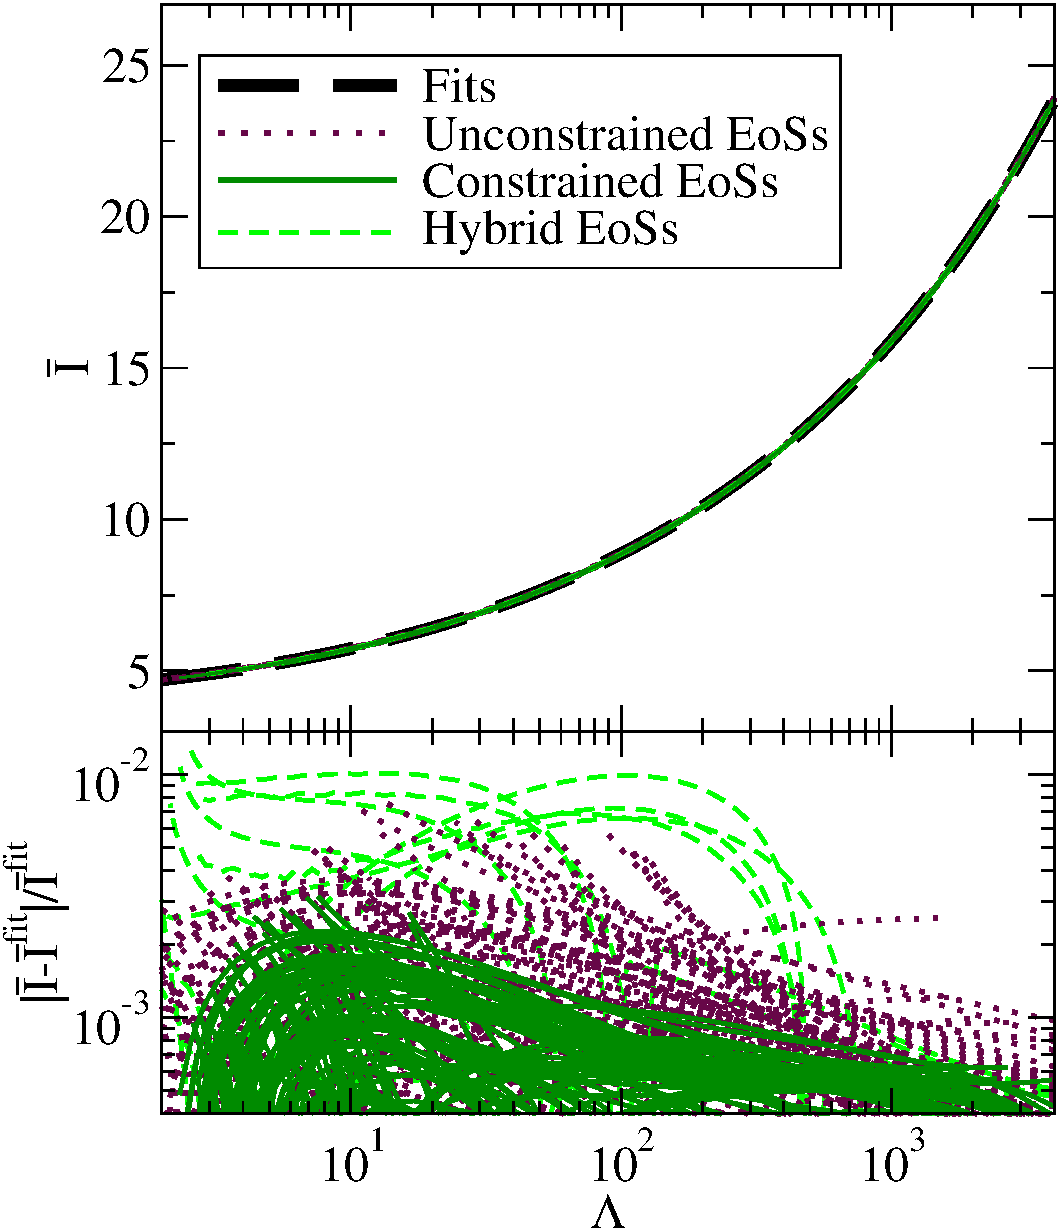
\includegraphics[width=.32\textwidth]{IL.pdf}
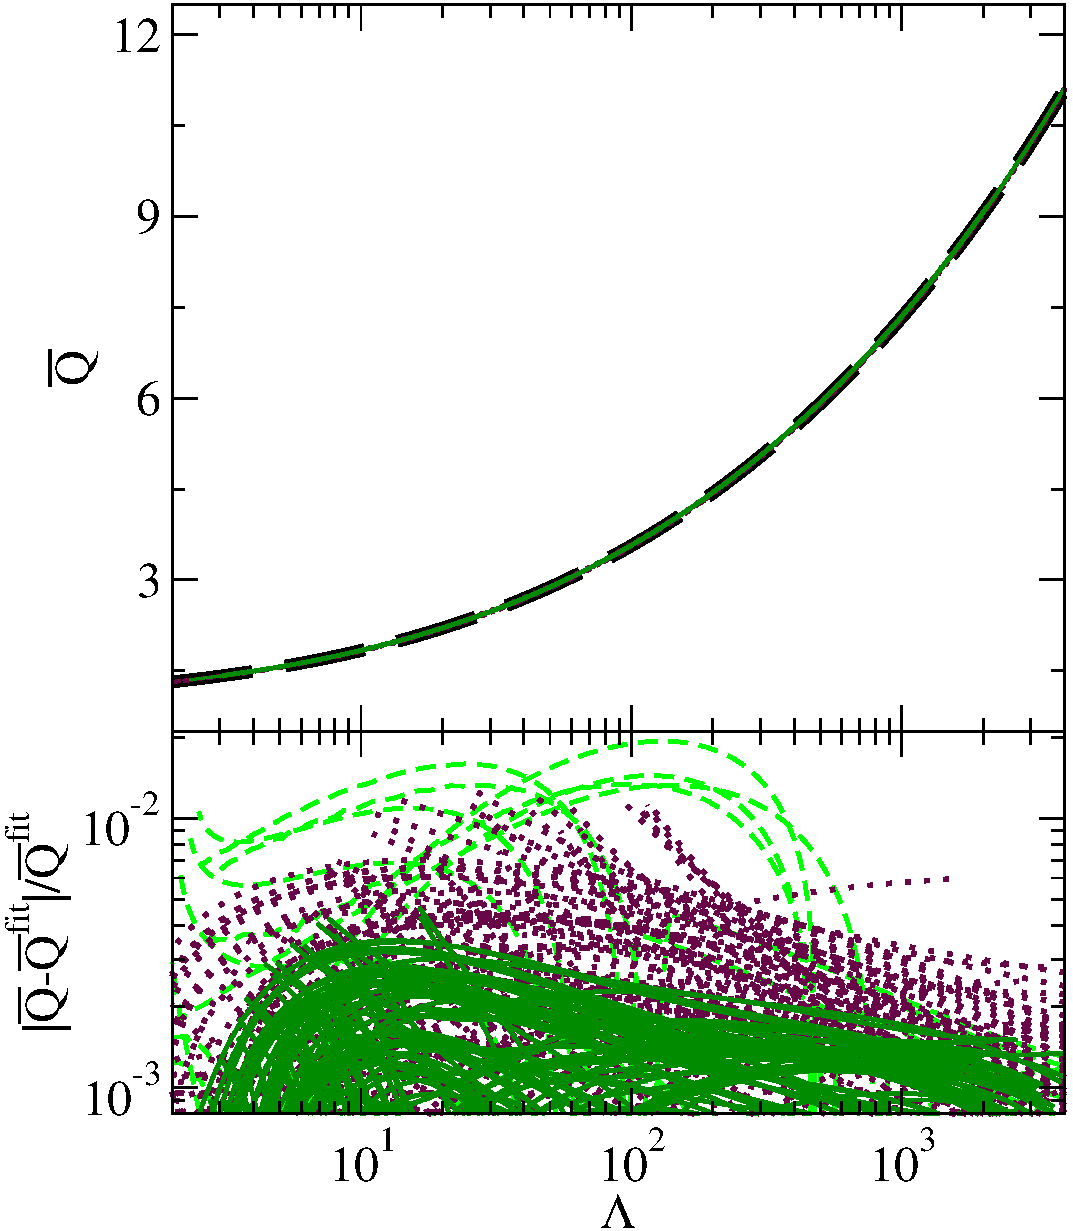
\includegraphics[width=.32\textwidth]{QL.pdf}
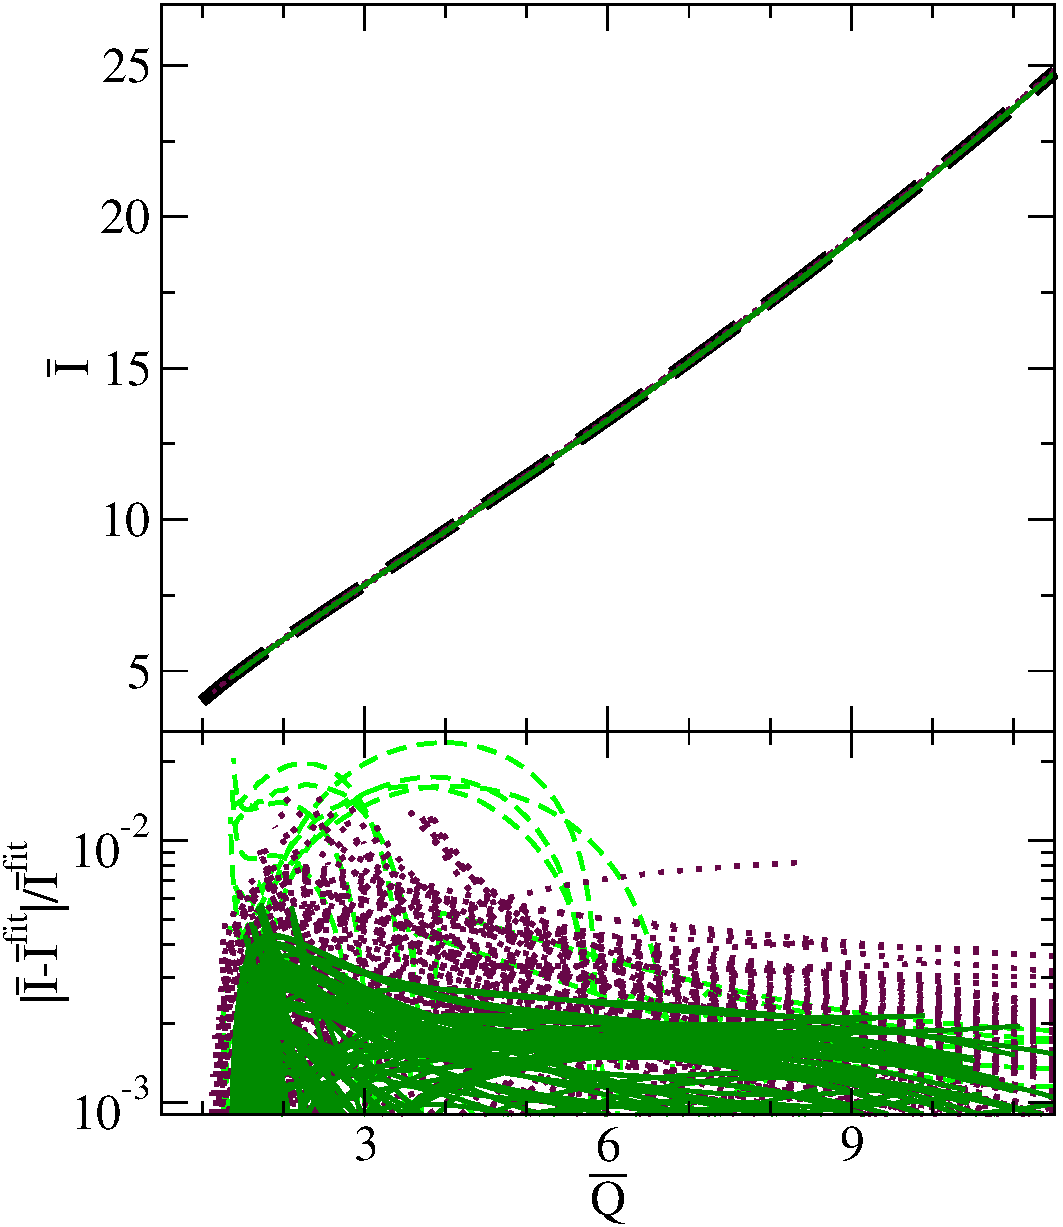
\includegraphics[width=.32\textwidth]{IQ.pdf}
\end{center}
\caption{
Individual I-Love-Q relations $\bar{I}-\Lambda$ (left), $\bar{Q}-\Lambda$ (center), and $\bar{I}-\bar{Q}$ (right), shown for both the constrained EoSs (solid green) and unconstrained EoSs (dotted maroon).
In these figures, the black dashed lines corresponds to the fits given by Eq.~\ref{eq:ILQfitNew}.
Observe how the fractional difference from the fits, shown in the bottom panels, is greatly suppressed for the constrained case, compared to both the unconstrained case, and results from previous works~\cite{Yagi:ILQ}.
The maximal EoS variation from the fits for the unconstrained and constrained sets of EoSs are compared in Tab.~\ref{tab:maxVar}.
Additionally shown in this figure is the fractional difference from the nuclear matter fits for the 10 hybrid star EoSs (dashed green).
}
\label{fig:ILQ}
\end{figure*} 


\begin{table}[htb]
\centering
\begin{tabular}{ c  || c c c } 
 \hline
 \hline
 \textbf{EoS-insensitive} & \multicolumn{3}{c}{\textbf{Maximal EoS Variability}} \\
 \cline{2-4}
 \textbf{Relation} & \multicolumn{1}{c|}{\emph{Previous}} & \multicolumn{1}{c|}{\emph{Unconstrained}} & \emph{Constrained}\\
 \hline
 $\bar{I}-\Lambda$ &  $0.0059$ & $0.0077$ & $0.0031$\\
 $\bar{Q}-\Lambda$ & $0.010$ & $0.013$ & $0.0047$\\
 $\bar{I}-\bar{Q}$ & $0.012$ & $0.015$ & $0.0057$\\
 \hline
 \multirow{2}{*}{$C-\Lambda$} & $0.065$ & $0.072$ & $0.022$\\
 & (--) & ($0.018$) & ($0.0066$)\\
  \hline
 \multirow{2}{*}{$R-\Lambda$} & -- & $0.056$ & $0.022$\\
 & (--) & ($880 \text{ m}$) & ($360 \text{ m}$) \\
 \hline
 $\Lambda_a-\Lambda_s$ & $\sim0.50$ & $0.57$ & $0.21$\\
 $q=0.90$ & (--) & ($190$) & ($37$) \\
 \cline{1-1}
 $\Lambda_a-\Lambda_s$ & $\sim0.20$ & $0.25$ & $0.083$\\
  $q=0.7$ & (--) & ($320$) & ($52$) \\
  \cline{1-1}
 $\Lambda_a-\Lambda_s$ & $\sim0.025$ & $0.038$ & $0.018$\\
  $q=0.50$ & (--) & ($240$) & ($29$) \\
  \cline{1-1}
\hline
\hline
\end{tabular}
\caption{Maximum relative and fractional EoS variation in the I-Love-Q, C-Love, R-Love, and binary Love relations using the unconstrained set, the constrained set and variations reported in previous work~\cite{Yagi:ILQ,Yagi:binLove}. The maximum absolute EoS variation is also reported in the C-Love, R-Love and binary Love cases in parenthesis. Observe that the maximum variation in the constrained set case is better than a factor of two smaller than the variability in the unconstrained case and in previous work. The maximum EoS variation in the unconstrained set is slightly larger than that found in previous work because the former is built from a large random sampling of EoSs.
}\label{tab:maxVar}
\end{table}

\subsubsection{Hybrid quark-hadron stars}
\label{sec:ilq-hyb}

Let us now focus on the I-Love-Q relations of hybrid stars, and their compatibility with their nuclear matter counterparts. For concreteness, we consider three different sets of EoSs in the hybrid case:
\begin{enumerate}
\item the complete set of 100 constrained EoSs combined with the 10 hybrid star EoSs,
\item the complete set of 100 constrained EoSs alone,
\item the complete set of 10 hybrid star EoSs alone.
\end{enumerate}
For each of these cases, we compute the I-Love-Q relations, we fit the data to Eq.~\eqref{eq:ILQfitNew} and we compute the relative fractional difference. 

\begin{table}[htb]
\centering
\begin{tabular}{ c  || c c } 
 \hline
 \hline
 \textbf{Fitting} & \multicolumn{2}{c}{\textbf{Maximal EoS Variability}} \\
 \cline{2-3}
 \textbf{Case} &  \multicolumn{1}{c|}{\emph{Constrained}} & \emph{Hybrid}\\
 \hline
 \emph{Combined} &  \multirow{2}{*}{$0.0044$} & \multirow{2}{*}{$0.014$}\\
 \emph{(Case 1)} & &\\
 \cline{1-1}
 \emph{Constrained only} & \multirow{2}{*}{$0.0031$} & \multirow{2}{*}{$0.017$}\\
  \emph{(Case 2)} & &\\
  \cline{1-1}
 \emph{Hybrid only} & \multirow{2}{*}{$0.0084$} & \multirow{2}{*}{$0.010$}\\
  \emph{(Case 3)} & &\\
  \cline{1-1}
\hline
\hline
\end{tabular}
\caption{
Maximum relative and fractional EoS variation in the I-Love relation, fitting to three different sets of data: using the constrained set plus hybrid EoSs, using the constrained set alone, EoS data alone, and using only the hybrid EoSs. In all 3 cases the hybrid EoSs are EoS-insensitive to $\sim1$\%, which is a slight decrease in universality relative to the hadronic only EoSs.
}\label{tab:hybridCompare}
\end{table}

The fractional differences for the second case (fit to only the constrained EoSs) is shown with dashed green lines in Fig.~\ref{fig:ILQ}, while the maximum EoS variation for the I-Love relation is shown in Table~\ref{tab:hybridCompare} for both the constrained and hybrid star cases. Observe how the hybrid star EoSs obey the I-Love-Q relations in each case to better than $\sim1.7$\%, a variability that is slightly higher than that found when using only nuclear matter EoSs in previous works~\cite{Yagi:ILQ}. Observe also that the universality cannot be improved much through the introduction of new fits, only bringing the maximal EoS variation down to $\sim1$\% for the fits constructed with only hybrid star EoSs. From this study, we conclude that hybrid star EoSs \emph{do} obey the traditional nuclear I-Love-Q relations computed with nuclear EoS data, albeit with a slight decrease in universality to $\sim1.7$\%.  

%%%%%%%%%%%%%%%%%%%%%%%%%%
%%%%%%%%%%%%%%%%%%%%%%%%%%
%%%% C-LOVE RELATIONS %%%%
%%%%%%%%%%%%%%%%%%%%%%%%%%
%%%%%%%%%%%%%%%%%%%%%%%%%%

\begin{figure*}
\begin{center} 
\includegraphics[width=\columnwidth]{CL.eps}
\includegraphics[width=\columnwidth]{RL.eps}
\end{center}
\caption{
Similar to Fig.~\ref{fig:ILQ} but for the C-Love (left) and the R-Love relations (right), with the bottom panels showing the \emph{absolute differences} (rather than fractional difference as in Fig.~\ref{fig:ILQ}) from the fit. Observe how the absolute difference is suppressed in the constrained set case relative to the unconstrained set, and results from previous work~\cite{Yagi:binLove}. In the left panel, we also present the C-Love relations in the hybrid star cases (dashed green) for comparison, where observe that, although still EoS-insensitive, the degree of universality decreases. {\ny{Why is the size of the right panel larger than the left panel?}}
}
\label{fig:clove}
\end{figure*} 

\subsection{C-Love Relations}
\label{sec:clove}

In this subsection we focus on the EoS-insensitive C-Love relations, as introduced by Yagi and Yunes in~\cite{Yagi:binLove}, as well as on the R-Love relations, since these play a key role in GW data analysis for the extraction of M-R credible intervals. As in the previous subsection, we consider both nuclear matter EoSs, as well as hybrid quark-hadron star EoSs.

\subsubsection{Nuclear matter stars}
\label{sec:clove-nuc}

Following Ref.~\cite{Yagi:binLove}, we begin by fitting the data for each set of EoSs to the simple curve
\begin{equation}
C = \sum^2_{k=0} a_k (\ln{\Lambda})^k.
\end{equation}
Doing so, yields $a_0 = 0.3617$, $a_1 = -0.03548$, and $a_2 = 0.0006194$, similar to what was found in~\cite{Yagi:binLove} {\ny{Wait, this is for the constrained set or the unconstrained set? I'm guessing you used the constrained set, but we should say so here.}}. As in the I-Love-Q case, however, the above fitting function does not limit properly to the Newtonian result 
\begin{equation}
C^N=K_{C\Lambda}\Lambda^{-1/5}.\label{eq:cloveFit}
\end{equation}
We thus repeat the fit using Eq.~\ref{eq:ILQfitNew} as the fitting function, with the new fitting coefficients presented in Table~\ref{tab:ILQfitNew}.

The left panel of Fig.~\ref{fig:clove} shows the C-Love relations for both the constrained and unconstrained sets, along with the corresponding \emph{absolute differences} from the fits (instead of the fractional differences as done back in Fig.~\ref{fig:ILQ}). Observe how the fit to the constrained EoSs suppresses the EoS variability compared to the fit to the unconstrained set, as well as that of previous works~\cite{Yagi:binLove}. The maximal EoS variation is compared between these three cases in Table~\ref{tab:maxVar}.

From the C-Love relations, we can also compute directly the R-Love relation using $R(\Lambda)=M/C(\Lambda)$ and for a fixed NS mass $M$. The right panel of Fig.~\ref{fig:clove} shows the R-Love relation for the constrained and unconstrained sets fixing $M=1.48\text{ M}_{\odot}$ at the observed value for one of the NSs in the GW170817 event, with the bottom panel showing the absolute difference of the data and the fits. Observe that the C-Love relations allow us to infer the NS radius to better than $\sim 350 \textrm{m} $ in the constrained case, while the error goes up to $1,000 \textrm{m}$ in the unconstrained case, as also tabulated in Table~\ref{tab:maxVar}. The systematic uncertainty in the radius using the constrained fit is thus comparable to the $\sim 140\textrm{m}$ systematic uncertainty in the radius due to the choice of EoS to model the crust~\cite{Gamba:2019kwu}. 


\subsubsection{Hybrid quark-hadron stars}
\label{sec:clove-hyb}

Let us now focus on whether the C-Love relations hold for hybrid stars. Much like in Sec.~\ref{sec:ilq-hyb}, we perform 3 separate fits: one to the constrained set plus 10 hybrid EoSs, another to the constrained set only, and a third to the 10 hybrid EoSs only. We then compare the EoS insensitivity in each case.

The left panel of Fig.~\ref{fig:clove} shows the C-Love relation when fitting only to the constrained set (dashed green curves). Observe how the C-Love relation for hybrid star remains EoS-insensitive, but the degree of universality is not as high as in the case of hadronic NSs. Table~\ref{tab:hybridCompareClove} compares the maximal EoS variability for the constrained and hybrid star EoSs fitting to the three data sets described above. As in Sec.~\ref{sec:ilq-hyb}, observe how the maximal EoS variation for hybrid stars fluctuates only slightly ($\sim 4.5\% - 7\%$) in each case.�From this, we conclude that hybrid stars do obey the C-Love relation derived for nuclear matter stars, with the caveat that the maximum universality increases to $\sim 7.1\%$.

\begin{table}
\centering
\begin{tabular}{ c  || c c } 
 \hline
 \hline
 \textbf{Fitting} & \multicolumn{2}{c}{\textbf{Maximal EoS Variability}} \\
 \cline{2-3}
 \textbf{Case} &  \multicolumn{1}{c|}{\emph{Constrained}} & \emph{Hybrid}\\
 \hline
 \emph{Combined} &  \multirow{2}{*}{$0.037$} & \multirow{2}{*}{$0.055$}\\
 \emph{(Case 1)} & &\\
 \cline{1-1}
 \emph{Constrained only} & \multirow{2}{*}{$0.022$} & \multirow{2}{*}{$0.072$}\\
  \emph{(Case 2)} & &\\
  \cline{1-1}
 \emph{Hybrid only} & \multirow{2}{*}{$0.058$} & \multirow{2}{*}{$0.045$}\\
  \emph{(Case 3)} & &\\
  \cline{1-1}
\hline
\hline
\end{tabular}
\caption{
Similar to Tab.~\ref{tab:hybridCompare} but for the C-Love relation.
Observe how for all 3 cases, the hybrid EoSs are only universal up to a minimum of $\sim1$\% (fractional difference from the fit), while in each case the constrained EoSs outperform the hybrid ones. The second case is also shown in Fig.~\ref{fig:clove}.
}\label{tab:hybridCompareClove}
\end{table}

%%%%%%%%%%%%%%%%%%%%%%%%%%%%%%%
%%%%%%%%%%%%%%%%%%%%%%%%%%%%%%%
%%%% BINARY LOVE RELATIONS %%%%
%%%%%%%%%%%%%%%%%%%%%%%%%%%%%%%
%%%%%%%%%%%%%%%%%%%%%%%%%%%%%%%

\subsection{Binary love relations}
\label{sec:binary}

\begin{figure}[htb]
\begin{center} 
\includegraphics[width=\columnwidth]{binLoveAbsolute.eps}
\end{center}
\caption{(Color online) Binary Love relations using Eq.~\ref{eq:binLovefit} fitted to the constrained (dotted maroon) and unconstrained sets (solid green), fixing $q=0.9$, $q=0.75$, and $q=0.50$. The bottom panels show the absolute difference (not the relative difference as in Fig.~\ref{fig:ILQ}) of the fit and the data. The fit to the constrained set shows a reduction in EoS variation relative to both the fit to the unconstrained set and previous work~\cite{Yagi:binLove}. For comparison, we also show the binary Love relations for the 10 hybrid star EoSs (dashed bright green curves), which present much larger EoS variation. 
}
\label{fig:binLove}
\end{figure} 

Let us now consider the binary Love relations. Following Ref.~\cite{Yagi:binLove}, we begin by fitting the binary Love relations to the constrained and unconstrained sets using the two-dimensional curve:
\begin{equation}\label{eq:binLovefit}
\Lambda_a=F_n(q) \frac{1+ \sum_{i=1}^3 \sum_{j=1}^2 b_{ij}q^j x^{i/5}}{1 + \sum_{i=1}^3 \sum_{j=1}^2 c_{ij}q^j x^{i/5}} \Lambda_s^{\alpha},
\end{equation}
where $q\equiv m_{1}/m_{2}$ is the mass ratio with $m_1 \leq m_2$, and $F_n(q)$ is the Newtonian-limiting controlling factor, given by
\begin{equation}\label{eq:control}
F_n(q) \equiv \frac{1-q^{10/(3-n)}}{1+q^{10/(3-n)}}.
\end{equation}
The coefficients of the fit to the constrained set are 
\begin{align}
b_{ij} = \begin{bmatrix}
    -14.40 & 14.45   \\
    31.36 & -32.25   \\
    -22.44 & 20.35   
\end{bmatrix}
\quad
c_{ij} = \begin{bmatrix}
    -15.25 & 15.37   \\
    37.33 & -43.20   \\
    -29.93 & 35.18   
\end{bmatrix},
\end{align}
{\ny{Zack, why did you pick a non-square matrix of coefficients to fit to? Typically, fits are better behaved when you stay with square matrices}}
and $n = 0.743$, where we set $\alpha = 1$ {\ny{Zack, is this right? I think you didn't fit for $\alpha$, but rather you set it to unity, but you did fit to $n$.  Please confirm.}} Unlike the individual I-Love-Q relations, the binary Love relations depend also depend on the mass ratio. 

Figure~\ref{fig:binLove} shows the improved binary Love relation for 3 different mass ratios ($q=0.9$, $q=0.75$, and $q=0.5$) for both the constrained and unconstrained sets of EoSs. Observe how, once again, the constrained set shows a considerable increase in EoS-insensitivity relative to both the unconstrained set and previous works~\cite{Yagi:binLove}. As before, the fit to the unconstrained set shows similar, yet slightly larger EoS variation than that found in previous work~\cite{Yagi:binLove} due to the random sampling used in our analysis. Observe that absolute error between the fit and the data is approximately independent of the mass ratio $q$, with a subtle maximum at $q=0.75$, which mimics the behavior of the controlling factor $F_n(q)$. As before, maximum EoS variation is tabulated in Tab.~\ref{tab:maxVar} for each value of mass ratio considered here.

We can extract two additional conclusions from from this Fig.~\ref{fig:binLove}. First, as the mass ratio becomes more extreme (i.e.~away from unity), the ranges of values that $\Lambda_s$ and $\Lambda_a$ can take decrease. This is because as $q$ decreases, there is a limited range of tidal deformabilities $\Lambda_{1,2}$ in the M-L relationships that satisfy the mass ratio constraint {\ny{What? I didn't understand the previous clause enough to rewrite it.}}, and thus, the allowed parameter space shrinks. Second, the fit to the constrained set does not extend to as high values of $\Lambda_s$ as the fit to the unconstrained set does. This is because of how the sets of EoSs were generated in our analysis, with the unconstrained set including some EoSs that are stiffer and and others that are softer than those constrained by the GW170817 event. This results in the unconstrained set  containing a larger range of tidal deformabilities $\Lambda_{1,2}$ (from both above and below) than the constrained set, which ultimately leads to a \emph{larger} range of $\Lambda_s=\frac{1}{2}(\Lambda_1+\Lambda_2)$ values.

Let us now consider the binary Love relations for hybrid stars. As described in Sec.~\ref{sec:theory}, transitional quark-hadron matter stars undergo strong first-order phase transitions at a transitional pressure $P_{\text{tr}}$, where the hadronic branch departs into a quark-matter branch at the corresponding transitional mass $M_{\text{tr}}$. These transitions result in two distinct types of NSs, based on their observed mass: (i) massive ($M \geq M_{\text{tr}}$) hybrid stars that have quark-matter inner cores and nuclear matter elsewhere (which recall we denote ``HS"); and (ii) low-mass ($M \leq M_{\text{tr}}$) hadronic stars with no internal transition to quark matter (which recall we denote ``NS"). We therefore expect the binary Love relations for hybrid stars to present behavior identical to their purely hadronic counterparts below the transitional mass (or correspondingly above a transitional $\Lambda_{s,\textrm{tr}}$), and very different behavior for higher masses (or correspondingly for smaller $\Lambda_{s,\textrm{tr}}$). 

This behavior is exactly what we observe in Fig.~\ref{fig:binLove} for the binary Love relations of hybrid stars. Indeed, contrary to the case of EoS-insensitive relations for isolated hadronic stars (I-Love-Q, C-Love, and R-Love) which remain moderately EoS-insensitive for all hybrid stars, the binary Love relations depart from their hadronic counterparts below some transitional $\Lambda_{s}$. This is because at low pressures ($\Lambda_s>\Lambda_{s,\textrm{tr}}$) the binary is purely of NS/NS type (with the EoS for both stars a member of the constrained set), but once the critical pressure is reached ($\Lambda_{s}<\Lambda_{s,\textrm{tr}}$), one or both stars transition into the hybrid branch, resulting in large reductions in tidal deformability, as shown in the left panel of Fig.~\ref{fig:clove}. When one star lies on the hadronic-matter branch while the other is on the quark-matter branch, the difference between tidal deformabilities becomes larger than expected for pure hadronic-matter stars. This results in large deviations in the sums and differences of tidal deformabilities $(\Lambda_1 \pm \Lambda_2)$, disrupting the overall universality and generating the large ``bump" in the binary Love relations for hybrid stars\footnote{This discrepancy is not present in the I-Love-Q and C-Love relations due to their single-star nature.} seen in Fig~\ref{fig:binLove}.

From this analysis, we conclude that binaries containing one or more hybrid stars do \emph{not} satisfy the same binary Love relations as binaries that contain only traditional nuclear matter stars. This does not imply, however, that more sophisticated binary Love relations cannot be constructed that will remain EoS-insensitive and able to model both types of binary systems. Such relations, however, would necessarily have to include (at least) one new parameter that determines the transition between the hadronic and the quark branches, such that the ``bump'' in the binary Love relations can be properly modeled. Work along these lines is outside the scope of this paper. 

%%%%%%%%%%%%%%%%%%%%%%%%%%%%%
%%%%%%%%%%%%%%%%%%%%%%%%%%%%%
%%%% FUTURE OBSERVATIONS %%%%
%%%%%%%%%%%%%%%%%%%%%%%%%%%%%
%%%%%%%%%%%%%%%%%%%%%%%%%%%%%

\section{Impact on future observations}
\label{sec:observations}

We have now shown that binary NS merger observations can help improve the EoS-insensitive relations, but the question remains: is it worth it?
Current interferometer sensitivities are not yet high enough to accurately constrain the dominant tidal parameter $\tilde{\Lambda}$.
For example, GW170817 was detected by LIGO observing run 2 (``O2")~\cite{aLIGO} and was able to constrain $\tilde{\Lambda}$ to a $90\%$ confidence interval centered at $\mu_{\tilde{\Lambda}}=395$ and with a width of 325 (or $\sigma_{\tilde{\Lambda}} \approx 198$).  This corresponds to statistical uncertainties of ${\cal{O}}(80\%)$, which dominates the error budget compared to the small systematic uncertainties picked up by EoS variation in the EoS-insensitive relations.
This implies that currently, the use of improved EoS-insensitive relations will only make a negligible difference on the extraction of tidal parameters.

In this section, we further explore this question and study when in the future the new set of improved relations will become important as current detectors are improved and new ones are built. In Sec.~\ref{sec:marginalization}, we first estimate the systematic uncertainties introduced by using the improved binary Love relations.
In Sec.~\ref{sec:futureObservations}, we estimate the statistical uncertainties on the extraction of tidal parameters, and compare them to the above-mentioned systematic uncertainties.
This is repeated for 5 future detectors, where multiple detections become important, but to combine constraints from multiple events we cannot use the $\tilde\Lambda$ parameterization, as this depends on the masses of the binary constituents. To remedy this, we re-parameterize the waveform in terms of the coefficients $\lambda_0$ (sometimes called $\Lambda_{1.4}$) and $\lambda_1$, obtained from a Taylor expansion of the dimensionless tidal deformability $\Lambda$ about a ``canonical" reference mass $M_0=1.4\text{ M}_{\odot}$~\cite{delPozzo:TaylorTidal,Yagi:binLove}:
\begin{equation}
\Lambda = \lambda_0 + \lambda_1 \left(1-\frac{M}{M_0}\right) + {\cal{O}}\left[\left(1-\frac{M_{0}}{M}\right)^{2}\right].
\end{equation}
The Taylor coefficients $\lambda_0$ and $\lambda_1$ are mass independent, and thus they are identical in all binary NS observations, and their posteriors may be combined.

\subsection{Marginalization over Uncertainties}\label{sec:marginalization}

Let us begin by investigating the residuals on $\Lambda_a(\Lambda_s,q)$ and the induced residuals on $\lambda_{0}$, in order to marginalize over the intrinsic uncertainty found in the binary Love relations.
In particular, we restrict our focus to only the constrained set of EoSs.
Residuals in $\Lambda_a$ are computed as $\Lambda_a^{\text{relation}}(\Lambda_s,q)-\Lambda_a^{\text{true}}$, where $\Lambda_a^{\text{true}}$ corresponds to the true value predicted by the sampled EoSs, and $\Lambda_a^{\text{relation}}(\Lambda_s,q)$ corresponds to the fit found in Sec.~\ref{sec:binary}.
We then convert the $\Lambda_a$ residuals into $\lambda_0$ residuals, as we describe below.

{\ny{Please rewrite everything from here to Subsection B. It is not clear at all what you've done, why you've done it, and what you got.}}
Following Ref.~\cite{Katerina:residuals}, we assume the residuals on $\Lambda_a$ observe a Gaussian distribution with mean and standard deviation given by:
\begin{align}
\mu_{\Lambda_a}(\Lambda_s,q) &=\frac{\mu_{\Lambda_s}(\Lambda_s)+\mu_{q}(q)}{2},\\ 
\sigma_{\Lambda_a} &=\sqrt{\sigma_{\Lambda_s}^2(\Lambda_s) + \sigma_{q}^2(q)}. 
\end{align}
%The mean and standard deviation of the Gaussian distribution of the residuals on 
We then fit the individual components using the following power functions {\ny{to what data? This is confusing}}:
\begin{align}
\mu_{\Lambda_s}(x) &= \mu_1 x + \mu_2, \label{eq:margFit1}\\ 
\mu_{q}(x) &= \mu_3 x^2 + \mu_4 x + \mu_5, \label{eq:margFit2}\\ 
\sigma_{\Lambda_s}(x) &= \sigma_1 x^{5/2} + \sigma_2 x^{3/2} + \sigma_3 x \sigma_4 x^{1/2} + \sigma_5, \label{eq:margFit3}\\ 
\sigma_{q}(x) &= \sigma_6 x^3 + \sigma_7 x^2 + \sigma_8 x + \sigma_9. \label{eq:margFit4}
\end{align}
The fitting parameters $\mu_i$ and $\sigma_i$ are tabulated in Table~\ref{tab:marginalized}.

\begin{table}
\centering
\addtolength{\tabcolsep}{1pt} 
\begin{tabular}{ c | c || c | c}
\hline 
\noalign{\smallskip}
$\mu_1$ & $3.509 \times 10^{-3}$ & $\sigma_1$ & $-2.074 \times 10^{-7}$\\
$\mu_2$ & $9.351 \times 10^{-1}$ & $\sigma_2$ & $-1.492 \times 10^{-3}$\\
$\mu_3$ & $-18.07$ & $\sigma_3$ & $-4.891 \times 10^{-2}$\\
$\mu_4$ & $27.56$ & $\sigma_4$ & $8.207 \times 10^{-1}$\\
$\mu_5$ & $-10.10$ & $\sigma_5$ & $-1.308$\\
 &  & $\sigma_6$ & $-63.76$\\
 &  & $\sigma_7$ & $11.14$\\
 &  & $\sigma_8$ & $75.25$\\
 &  & $\sigma_8$ & $-23.69$\\
 \noalign{\smallskip}
 \hline
\end{tabular}
\caption{
Coefficients to the fits given by Eqs.~(\ref{eq:margFit1})-(\ref{eq:margFit4}) for the relative error on $\Lambda_a$ in the improved binary Love EoS-insensitive relations presented in this paper.
}\label{tab:marginalized}
\addtolength{\tabcolsep}{-1pt}
\end{table}

Now that we have obtained the residuals on $\Lambda_a$, we must convert them into residuals on the new tidal parameter $\lambda_0$, in order to compute and easily compare the systematic uncertainties to the statistical uncertainties on $\lambda_0$. {\ny{You need to say explicitly how you did this.}}
Figure~\ref{fig:qLsResiduals} shows the standard deviations of these residuals (converted into $\lambda_0$) binned in both $q$ and $\Lambda_s$. 
To estimate the overall systematic uncertainties on $\lambda_0$ accrued upon the use of the improved binary Love relations, we combine the uncertainties in both $q$ and $\Lambda_s$.
Figure~\ref{fig:residuals} displays the un-binned Gaussian distribution of $\lambda_0$ residuals for both the constrained, and unconstrained sets of EoSs for comparison.
Observe how the standard deviations $\sigma=9.764$ and $\sigma=78.28$ show a large decrease from the unconstrained to the constrained sets of EoSs.
Additionally, we find the 90th, 99th, and 100th percentiles on $\lambda_0$ to be $P_{90}=13.19$, $P_{99}=42.38$, and $P_{100}=111.32$ for the constrained EoSs.
Because the un-binned residuals seen in Fig.~\ref{fig:residuals} are dominated by the low-error regions of the parameter space ($\Lambda_s \rightarrow 0$, $\Lambda_s \rightarrow \infty$, $q \rightarrow 0$ and $q \rightarrow 1$) shown by Fig.~\ref{fig:qLsResiduals}, we consider the 90th percentile uncertainty (indicated by the dashed green line in Fig.~\ref{fig:qLsResiduals}) for the remainder of the analysis, in order to further take into account the high-error regions of the parameter space ($\Lambda_s \sim 2000$, $q\sim0.5$).
We take this value of $P_{90}=13.19$ to be the systematic measurement uncertainty introduced by using the improved binary Love relations on the parameter extraction of $\lambda_0$, indicated by the dashed indigo line in Fig.~\ref{fig:stackedFisher}.
Similarly, we derive the systematic measurement uncertainty on $\tilde\Lambda$ to be $12.01$, shown in Fig.~\ref{fig:singleFisherLt}.
Currently, the statistical uncertainty of $170.1$ on $\lambda_0$ from GW170817 dominates the error budget compared to the systematic uncertainty of $13.19$, as seen in Fig.~\ref{fig:stackedFisher}.
This means that, for the current ``O2" detector sensitivity, the use of improved binary Love relations will only make a negligible difference on the extraction of $\tilde\Lambda$.
However, future detectors (for example aLIGO, A\texttt{+}, Voyager, CE, and ET) are planned with large reductions in sensitivity - both decreasing the statistical uncertainties and allowing for larger binary NS merger detection rates; further reducing the statistical uncertainties.
In Sec.~\ref{sec:futureObservations}, we analyze this further and discuss when the systematic uncertainties from EoS-insensitive relations become comparable to the statistical uncertainties.

\begin{figure}
\begin{center} 
\includegraphics[width=\columnwidth]{qResiduals.eps}
\includegraphics[width=\columnwidth]{LsResiduals.eps}
\end{center}
\caption{$\lambda_0$ residuals binned in $q$ (top) and $\Lambda_s$ (bottom), highlighting the different error weights across the entire $(q,\Lambda_s)$ parameter space.
In this figure, the violet circles indicate the standard deviation of each bin in $q$-space ($\Lambda_s$-space), while the solid black lines represent the best fit given by Eqs. (\ref{eq:margFit3})-(\ref{eq:margFit4}).
Observe how the uncertainty is maximal for $q\sim0.5$ and $\Lambda_s\sim2000$, while it becomes minimal for both low and high values of $q$ and $\Lambda_s$.
Also shown in the figure is the 90th percentile of the un-binned residuals seen in Fig.~\ref{fig:residuals}, taken to be the overall systematic uncertainty introduced by using binary Love relations.
}
\label{fig:qLsResiduals}
\end{figure}

\begin{figure}
\begin{center} 
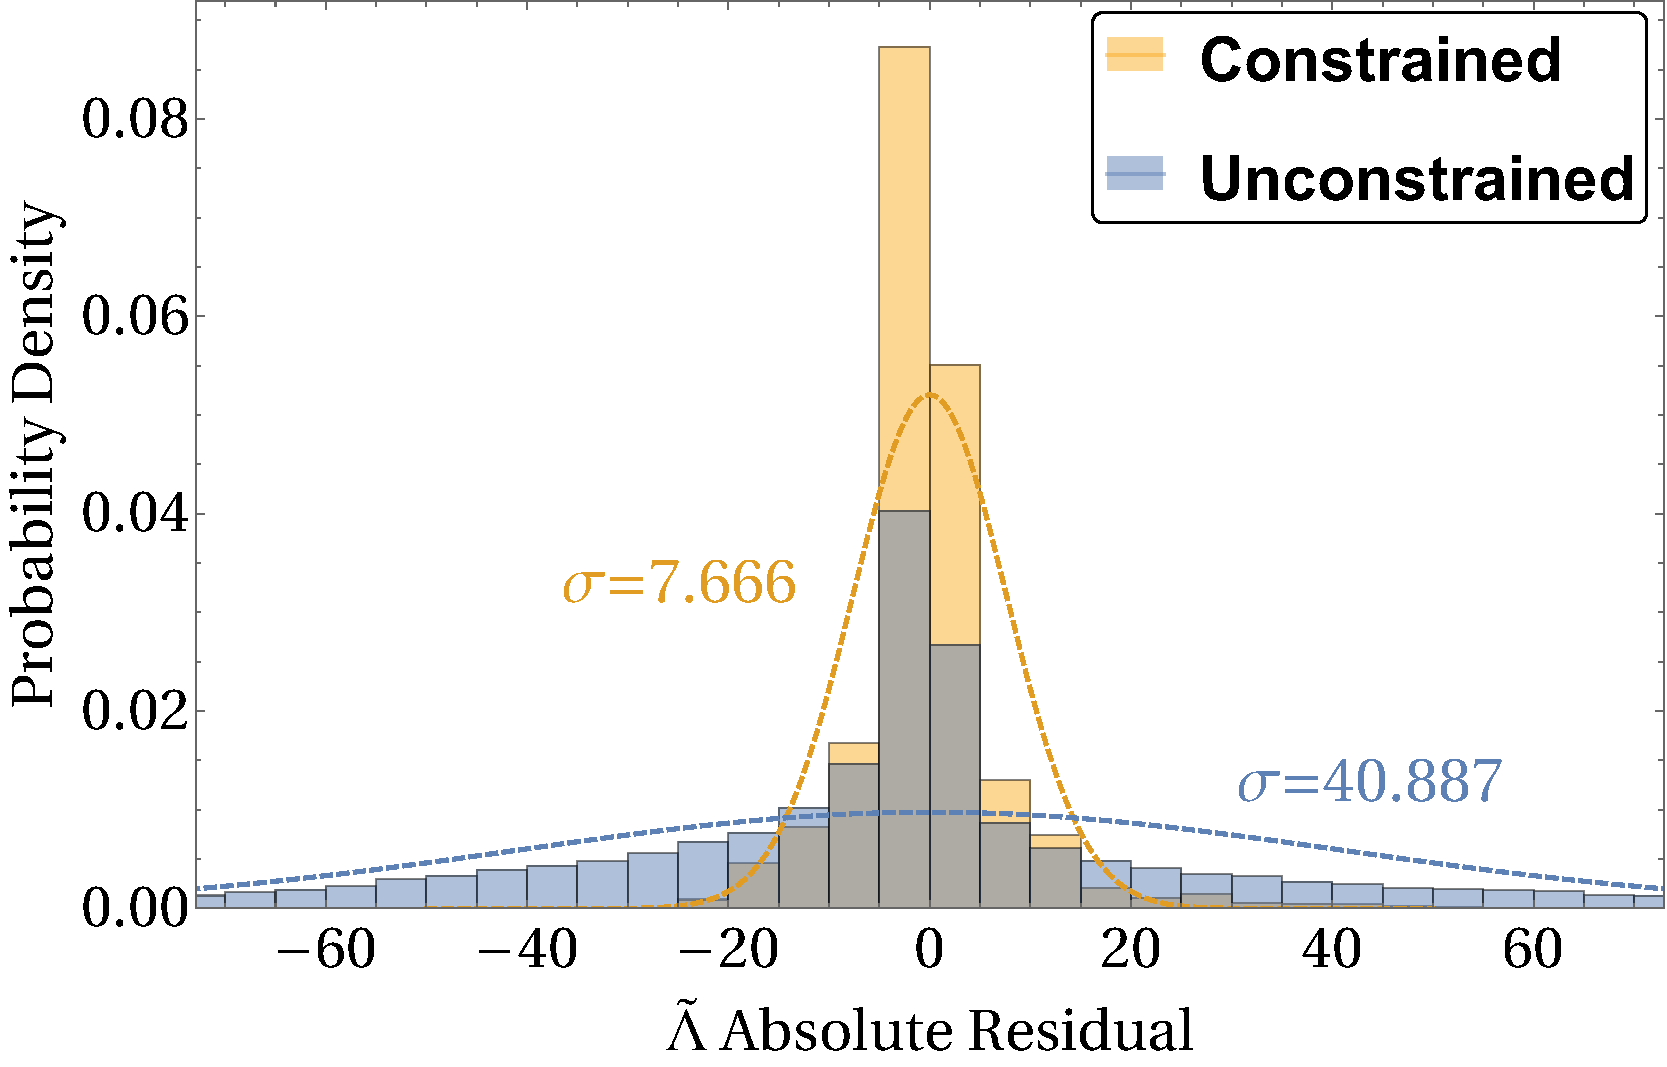
\includegraphics[width=\columnwidth]{residuals.pdf}
\end{center}
\caption{
Residuals on $\lambda_0$ computed as $\lambda_0^{\text{fit}}-\lambda_0^{\text{true}}$ for the binary Love relations modeled in Sec.~\ref{sec:binary} for both constrained and unconstrained sets of EoSs.
These residuals obey Gaussian distributions centered at $\mu=-0.1530$ and $\mu=0.2710$ with standard deviations of $\sigma=9.764$ and $\sigma=78.28$ for the constrained and unconstrained sets of EoSs, respectively.
These uncertainties correspond roughly to the systematic uncertainties introduced on the parameter extraction of $\lambda_0$ upon the use of binary Love relations.
However, to take into account the systematic uncertainties found in high-error regions of the parameter space, we instead set the systematic uncertainty to be the 90th percentile, $P_{90}=13.19$.
Observe that the systematic uncertainties from using the improved (constrained) binary Love relations are negligible compared to the statistical uncertainties accrued on parameter extraction from GW170817, found to be $\sigma_{\lambda_0}=170.1$.
}
\label{fig:residuals}
\end{figure}

\subsection{Future Observations}\label{sec:futureObservations}

We now estimate the feasibility of using the improved EoS-insensitive relations in future GW observations of the coalescence of binary NSs. We estimate the statistical accuracy to which parameters can be extracted through a simple Fisher analysis~\cite{Finn:Fisher,Cutler:Fisher}, assuming sufficiently high signal-to-noise ratio and Gaussian noise~\cite{Cutler:Fisher,Berti:Fisher,Poisson:Fisher}. Henceforth, we consider a waveform template parametrized in terms of
\begin{equation}\label{eq:template}
\theta^a=(\ln{A},\phi_c,t_c,\ln{\mathcal{M}},\ln{\mathcal{\eta}},\chi_s,\chi_a,\lambda_0, \lambda_1),
\end{equation}
where $\eta \equiv m_1 m_2/m^2$ is the symmetric mass ratio with $m_{1,2}$ and $m$ being the individual and total masses, $\mathcal{M}=m \eta^{3/5}$ is the chirp mass, $A \equiv {\mathcal{M}^{5/6}}/({\sqrt{30}\pi^{2/3}D_L})$ is a normalized amplitude factor with $D_L$ the luminosity distance, and $\chi_{s,a}=\frac{1}{2}(\chi_1\pm\chi_2)$ are the symmetric and antisymmetric dimensionless spin parameters. The resulting posterior distribution is Gaussian with a root-mean-square given by:
\begin{equation}
\Delta \theta^a=\sqrt{\Big( \tilde{\Gamma}^{-1}\Big)^{aa}}.
\end{equation}
Here, the Fisher matrix $\tilde{\Gamma}$ is defined by:
\begin{equation}
\tilde{\Gamma}_{ab} \equiv \Big( \frac{\partial h}{\partial \theta^a} \Big| \frac{\partial h}{\partial \theta^a}\Big) + \frac{1}{\sigma_{\theta^a}^2} \delta_{ab}
\end{equation}
where $h$ is the waveform template, $\sigma_{\theta^a}$ are the parameters' prior root-mean-square estimate, and the inner product is defined by:
\begin{equation}
(a|b) \equiv 2 \int^{\infty}_0\frac{\tilde{a}^*\tilde{b}+\tilde{b}^*\tilde{a}}{S_n(f)}df.
\end{equation}

In this analysis, we consider the ``PhenomD" (IMRD) waveform template~\cite{PhenomDI,PhenomDII} modified by two different tidal corrections: the 6PN tidal correction shown in Ref.~\cite{Wade:tidalCorrections} (IMRD + 6PN), and the NRTidal correction shown in Ref.~\cite{Samajdar:NRTidal} (IMRD + NRTidal).
Comparing the two different tidal corrections to the IMRD waveform returns a rough estimate on the magnitude of waveform mismodeling systematics.
Lastly, we consider the spectral noise densities $S_n^A(f)$ for 6 different interferometer designs: $A \equiv ($O2~\cite{aLIGO}, aLIGO~\cite{aLIGO}, A\texttt{+}~\cite{Ap_Voyager_CE}, Voyager~\cite{Ap_Voyager_CE}, CE~\cite{ET}, ET-D~\cite{Ap_Voyager_CE}$)$ in order to compare the statistical uncertainties accrued on parameter extraction using future upgraded LIGO detectors as well as third generation detectors.

We begin by authenticating this approach by applying a Fisher analysis (with an IMRD + 6PN waveform injection) to GW170817, as observed by LIGO with O2 detector sensitivity~\cite{aLIGO}.
Because only 1 event was detected, we utilize $\tilde\Lambda$ and $\delta\tilde\Lambda$ as the tidal parameters for comparison purposes.
Further, we scale the luminosity distance such that the signal-to-noise-ratio ($SNR \equiv \rho$) is fixed to be $\rho=32.4$, as was found in GW170817.
We also assume low spin priors $|\chi| \leq 0.05$, as well as $\tilde{\Lambda} \leq 3000$ and $|\delta \tilde{\Lambda}| \leq 500$~\cite{Wade:LambdaPriors}.
The resulting posterior distribution on $\tilde{\Lambda}$ has a range of $\pm 276.99$ encompassing the $90\%$ credible levels.
We compare these results with the Bayesian analysis performed in Ref.~\cite{TheLIGOScientific:2017qsa,Abbott2018}, finding close agreement with the resulting $90\%$ credible region of $70 \leq \tilde{\Lambda} \leq 720$.
This confirms the approximate validity of this method, allowing a continuation of this analysis for future detectors.
\begin{figure}
\begin{center} 
\includegraphics[width=\columnwidth]{sensitivities.eps}
\end{center}
\caption{
Square root of of the spectral noise densities $\sqrt{S_n^A(f)}$ plotted for detectors ($A$): LIGO O2, aLIGO, A\texttt{+}, Voyager, CE, and ET-D as interpolated from publicly available data.
Spectral noise densities are plotted from $f_{\text{min}}=(23,10,10,7,1,1) \text{ Hz}$, respectively, to $f_{\text{max}}=1649 \text{ Hz}$.
Also shown is $2 \sqrt{f}$ multiplied by the amplitude of the PhenomD~\cite{PhenomDI,PhenomDII} waveform template.
}
\label{fig:sensitivities}
\end{figure}

Next, we consider events identical to GW170817 detected on future design sensitivity upgrades and detectors $A \equiv ($O2, aLIGO, A\texttt{+}, Voyager, CE, ET-D$)$, shown in Fig.~\ref{fig:sensitivities}.
Further, we consider the combined statistical uncertainties of $N_A$ events detected over 1 year on detector $A$, determined by integrating the local binary NS (BNS) merger rate over redshifts up to the horizon redshift of each detector.
Here we assume low spin priors $|\chi| \leq 0.05$, as well as $0 \leq \lambda_0 \leq 3207$ and $-4490 \leq \lambda_1 \leq 0$~\cite{delPozzo:TaylorTidal}\footnote{These are converted from the dimensional forms found in Ref.~\cite{delPozzo:TaylorTidal} into their corresponding dimensionless forms.}.
The process we utilize to compute single and combined statistical uncertainties for each detector sensitivity $S_n^A(f)$ is detailed in App.~\ref{app:stackingProcedure}.
From this, we determine if and when the statistical uncertainties associated with the parameter extraction of $\lambda_0$ drop below the systematic EoS variation errors from using binary Love relations.

The results for this process upon the injection of the IMRD + 6PN waveform are compiled in Table~\ref{tab:variances}, and shown graphically in Fig.~\ref{fig:stackedFisher} where $\sigma^A_{\text{GW170817}}$ and $\sigma^A_N$ are plotted as a function of $\rho^A_{\text{GW170817}}$ (the SNR as if GW170817 were detected on future detector $A$) for 5 future detector sensitivities.
For reference, Fig.~\ref{fig:singleFisherLt} also displays the estimated $\tilde\Lambda$ extraction efficiency for \emph{one} event on each detector; as these events can not be combined like was done in the case of $\lambda_0$.
Observe how this figure shows similar results on $\tilde\Lambda$ to that found on $\lambda_0$ for the case of one event - that is, future third-generation detectors ET and CE both observe statistical uncertainties on $\tilde\Lambda$ (and $\lambda_0$) dropping below the systematic binary Love errors for a single event.
This result is amplified when multiple events are combined as shown in Fig.~\ref{fig:stackedFisher}, further motivating the need to improve the systematic uncertainties in the binary Love relations for upcoming detectors Voyager, CE and ET.
We note that in Figs.~\ref{fig:stackedFisher} and~\ref{fig:singleFisherLt}, the single-event measurement uncertainties are slightly larger for CE than for ET despite having a larger SNR.
This relic originates from the high-frequency dependence of CE and ETs detector sensitivities: due to the 3-detector geometry of ET, it is able to more accurately measure the tidal effects emergent at high frequencies.
However, when computing the SNRs from $1 \text{ Hz} \leq f \leq 1649 \text{ Hz}$, CE dominates over ET and observes a larger SNR.
When instead setting the minimum frequency to $f_{\text{min}} \geq 68$ Hz however, the SNR for ET instead dominates that for CE, validating our hypothesis on this effect.

\begin{figure}
\begin{center} 
\includegraphics[width=\columnwidth]{singleFisherLt.eps}
\end{center}
\caption{
Estimated statistical uncertainties $\sigma^A_{\text{GW170817}}$ in the extraction of $\tilde\Lambda$ from GW170817 (O2) as if observed with future interferometers aLIGO, A\texttt{+}, Voyager, CE, and ET-D as a function of the signal-to-noise-ratio $\rho^A_{\text{GW170817}}$.
Also shown is the systematic uncertainty on $\tilde\Lambda$ derived using the same method used to compute the systematic uncertainty on $\lambda_0$.
This is similar to Fig.~\ref{fig:stackedFisher} where the extraction efficiency of $\lambda_0$ was plotted, however, in this case multiple events can \emph{not} be combined due to the variation in mass and therefore $\tilde\Lambda$ among events.
}
\label{fig:singleFisherLt}
\end{figure} 

\begin{table*}
\centering
\caption{
Tabulated results for the estimated statistical uncertainties on the tidal deformability at $1.4\text{ M}_{\odot}$, $\lambda_0$, for the combined results of $N_A$ detections corresponding to the estimated upper, central, and lower limits of the binary NS merger detection rate $\mathcal{R}$.
This is repeated for 5 future detector sensitivities: aLIGO, A\texttt{+}, Voyager, CE, and ET.
Below, $\rho^A_{\text{GW170817}}$ and $\sigma^A_{\text{GW170817}}$ correspond to the approximate SNR and $\sigma_{\lambda_0}$ of GW170817 had it been observed by future interferometer $A$, and $\sigma^A_N$ corresponds to the overall uncertainty on $\lambda_0$ after $N_A$ detections on interferometer $A$.
It can be seen here that the statistical uncertainties on $\lambda_0$ become comparable with the systematics (set to be $P_{90}=13.19$) from using improved binary Love relations for future detectors Voyager, ET, and CE, indicating when it will become important to improve the EoS-insensitive relations.
Note that the approximation for $\sigma^A_N$ under the O2 detector sensitivity is left blank due to the singularity of the detected event.
These results are also shown graphically in Fig.~\ref{fig:stackedFisher}.
}\label{tab:variances}
\begin{tabular}{|c|@{\extracolsep{4pt}}c@{\extracolsep{0pt}}|c|@{\extracolsep{4pt}}C{1.7cm}@{\extracolsep{-2pt}}|C{1.7cm}|@{\extracolsep{-2pt}}C{1.7cm}@{\extracolsep{2pt}}|c|@{\extracolsep{0pt}}c@{\extracolsep{0pt}}|c|}
\cline{1-1}\cline{2-3}\cline{4-9}
    \multicolumn{1}{|c|}{\bfseries Detectors (A)} & \multicolumn{2}{|c|}{\bfseries GW170817} & \multicolumn{6}{|c|}{\bfseries Multiple events} \\
\cline{1-1}\cline{2-3}\cline{4-9}
\noalign{\smallskip}
\cline{2-3}\cline{4-6}\cline{7-9}
\multicolumn{1}{c}{} & \multicolumn{1}{|c|}{} & \multicolumn{1}{c|}{} & \multicolumn{3}{|c|}{} & \multicolumn{3}{|c|}{}
\\[-1em]
\multicolumn{1}{c}{}  &  \multicolumn{1}{|c|}{\multirow{2}{*}{$\rho^A_{\text{GW170817}}$}}  &  \multirow{ 2}{*}{$\sigma^A_{\text{GW170817}}$}  &  \multicolumn{3}{|c|}{$N_A$}  &  \multicolumn{3}{|c|}{$\sigma^A_N$}  \\
\cline{4-6}\cline{7-9}
\multicolumn{1}{c}{}  &  \multicolumn{1}{|c|}{}  &  \multicolumn{1}{c|}{}  &  \multicolumn{1}{|c|}{Low}  &  \multicolumn{1}{c|}{Central} &  \multicolumn{1}{c|}{High}  & \multicolumn{1}{|c|}{Low}  &  \multicolumn{1}{c|}{Central} &  \multicolumn{1}{c|}{High}\\
\cline{2-3}\cline{4-6}\cline{7-9}
\noalign{\smallskip}
\noalign{\smallskip}
\cline{1-1}\cline{2-3}\cline{4-6}\cline{7-9}
 O2  & \multicolumn{1}{|c|}{$32.40$}  & $170.13$ &  \multicolumn{1}{|c|}{--} & -- & -- & \multicolumn{1}{|c|}{--} & -- & --\\
\cline{1-1}\cline{2-3}\cline{4-6}\cline{7-9}
 aLIGO  & \multicolumn{1}{|c|}{$90.74$}  & $109.7$ &  \multicolumn{1}{|c|}{$20$} & $98$ & $304$ & \multicolumn{1}{|c|}{$182.8$} & $83.31$ & $46.95$\\
\cline{1-1}\cline{2-3}\cline{4-6}\cline{7-9}
 A\texttt{+}  & \multicolumn{1}{|c|}{$180.95$}  & $45.64$ &  \multicolumn{1}{|c|}{163} & 786 & 2,419 & \multicolumn{1}{|c|}{$58.94$} & $24.69$ & $13.66$\\
\cline{1-1}\cline{2-3}\cline{4-6}\cline{7-9}

\multicolumn{1}{|c|}{} & \multicolumn{1}{|c|}{} & \multicolumn{1}{c|}{} & \multicolumn{1}{|c|}{} & \multicolumn{1}{c|}{} & \multicolumn{1}{c|}{} & \multicolumn{1}{|c|}{} & \multicolumn{1}{c|}{} & \multicolumn{1}{c|}{}
\\[-1em]

 Voyager  & \multicolumn{1}{|c|}{$428.89$}  & $25.26$ &  \multicolumn{1}{|c|}{2,191} & 10,544 & 32,454 & \multicolumn{1}{|c|}{$20.97$} & $9.556$ & $5.323$\\
\cline{1-1}\cline{2-3}\cline{4-6}\cline{7-9}

\multicolumn{1}{|c|}{} & \multicolumn{1}{|c|}{} & \multicolumn{1}{c|}{} & \multicolumn{1}{|c|}{} & \multicolumn{1}{c|}{} & \multicolumn{1}{c|}{} & \multicolumn{1}{|c|}{} & \multicolumn{1}{c|}{} & \multicolumn{1}{c|}{}
\\[-1em]

 ET-D  & \multicolumn{1}{|c|}{$1398.03$}  & $6.871$ &  \multicolumn{1}{|c|}{71,536} & 344,270 & 1,059,638 & \multicolumn{1}{|c|}{$3.848$} & $1.732$ & $0.9621$\\
\cline{1-1}\cline{2-3}\cline{4-6}\cline{7-9}

\multicolumn{1}{|c|}{} & \multicolumn{1}{|c|}{} & \multicolumn{1}{c|}{} & \multicolumn{1}{|c|}{} & \multicolumn{1}{c|}{} & \multicolumn{1}{c|}{} & \multicolumn{1}{|c|}{} & \multicolumn{1}{c|}{} & \multicolumn{1}{c|}{}
\\[-1em]

 CE  & \multicolumn{1}{|c|}{$2807.45$}  & $7.664$ &  \multicolumn{1}{|c|}{295,200} & 1,420,650 & 4,372,653 & \multicolumn{1}{|c|}{$3.720$} & $1.668$ & $0.8979$\\
\cline{1-1}\cline{2-3}\cline{4-6}\cline{7-9}
\end{tabular}
\end{table*}

Next, we repeat the process upon the injection of the IMRD + NRTidal waveform in order to demonstrate the effect of waveform mismodeling.
The results are shown in Fig.~\ref{fig:stackedFisher} as maroon outlined circles (single detection uncertainties) and an outlined dashed maroon region (combined uncertainties from multiple detections).
Observe the noticeable difference between the extraction efficiencies for the two different tidal corrections - highlighting the need for further waveform modeling for future interferometers.

Concluding, we find that the Voyager, ET, and CE detectors all exhibit enough statistical uncertainty reduction that the systematics on $\lambda_0$ and $\tilde\Lambda$ introduced from using improved EoS-insensitive relations (found to be $13.19$ and $12.01$, respectively) no longer become negligible in the error budget.
This implies that the use and further improvement of EoS-insensitive relations is not only justified, but necessary, for future binary NS merger detections.
Additionally, we find that the effect of waveform mismodeling is indeed important for future observations as the statistical uncertainties continue to decrease.
In Appendix~\ref{app:measurement}, we additionally investigate the dependence of the measurement accuracy on $\tilde\Lambda$ on the binary NS mass ratio $q$ for fixed chirp mass $\mathcal{M}=1.88\text{ M}_{\odot}$.

%%%%%%%%%%%%%%%%%%%%
%%%%%%%%%%%%%%%%%%%%
%%%% DISCUSSION %%%%
%%%%%%%%%%%%%%%%%%%%
%%%%%%%%%%%%%%%%%%%%

\section{Conclusion and Discussion}
\label{sec:conclusion}

The recent GW observation of binary NS merger GW170817 placed constraints on the supranuclear matter EoS for NSs.
We take advantage of this by generating a restricted set of spectral EoSs which agree with this observation in order to reduce the uncertainties upon the extraction of tidal parameters from future GW events.
Important previous work by Yagi and Yunes~\cite{Yagi:ILQ,Yagi:binLove} found EoS-insensitive relations between symmetric and antisymmetric combinations of NS tidal deformabilities, which aid in the extraction of said tidal parameters.
We find an improvement upon these EoS-insensitive relations by a factor of $\sim 59$\% for stars with mass ratios of $0.75$ by restricting to the EoS posterior samples from GW170817s 90\% credible region on pressure as a function of density.
Similarly, we find an increase in C-Love and I-Love-Q universality by factors of $\sim 76$\% and $\sim 50$\%, respectively.
These improvements on the I-Love-Q and C-Love relations can be very beneficial in many important analyses, including that done in Ref.~\cite{Kumar:2019xgp}, where constraints on the moment of inertia, tidal deformability, compactness, spin, and radius were found using such relations.
We also show the relationship between the NS radius and its tidal deformability, computed directly from the C-Love relations.
We find this relation to display a maximum uncertainty of $358.9\text{ m}$ from the fit discussed in Sec.~\ref{sec:clove}.
Additionally, we find that hybrid quark-hadron star EoSs \emph{do} obey the I-Love-Q and C-Love relations, albeit with slightly higher maximum EoS variabilities as displayed in Tabs.~\ref{tab:hybridCompare} and ~\ref{tab:hybridCompareClove}.
We additionally find that binaries consisting of one massive hybrid quark-hadron star, and one small-mass hadron star do not obey the binary Love relations -- explained by the large difference in $\tilde{\Lambda}$ displayed between the constituent stars.
From this we state that the hybrid star EoSs do \emph{not} obey the binary Love relations.
Future work currently in progress will attempt to remedy this through a series of new piecewise hybrid star binary Love relations.

In the second half of this paper, we analyze the impact of this improvement for future binary NS merger detections.
Currently detectors are not yet sensitive enough to accurately constrain $\tilde{\Lambda}$ for the improved EoS-insensitive relations to make a difference.
We find that future interferometers Voyager, CE, and ET-D all experience a reduction in the statistical uncertainties upon the extraction of $\tilde{\Lambda}$ enough to become comparable to the systematic uncertainties injected through the use of improved EoS-insensitive relations, as depicted in Fig.~\ref{fig:stackedFisher} and Table~\ref{tab:variances}.
Additionally, we considered the effect of waveform mismodeling by comparing Fisher analyses using two different tidal corrections to the PhenomD waveform: 6PN and NRTidal.
Doing so revealed a noticeable difference between the extraction uncertainties derived under injection of each waveform - indicating the need for further waveform modeling.
Finally, in Appendix~\ref{app:measurement} we investigate the effect of NS binary mass ratio q on the measurement accuracy of $\tilde\Lambda$.
We find that the second generation interferometers lose accuracy as one increases the mass ratio, while the third generation detectors observe a large increase in accuracy due to the correlations between $\tilde\Lambda$ and $\delta\tilde\Lambda$.
This indicates that the use and further improvement of EoS-insensitive relations is justified for future GW observations of binary NS merger events.

Future work on this subject entails an investigation into the improvement of alternative EoS-insensitive relations, such as the multipole Love relations between various $l$-th order electric, magnetic, and shape tidal deformabilities as discussed in Ref.~\cite{Yagi:Multipole}.
Additionally, Lackey \emph{et al}. presented surrogate models of non-spinning effective-one-body waveform models with the the use of universal relations in Refs.~\cite{Lackey:Surrogate, Lackey:EOB}.
By reducing the number of required waveform model parameters, surrogate models aid in the extraction of NS observables from GW detections.
The improvement in the multipole love relations can then be used to increase the accuracy of such surrogate models.
Additionally, we plan on a more comprehensive analysis into the intricacies of new hybrid star binary Love relations, as discussed in Sec.~\ref{sec:binary}.
Work along this direction is currently in progress.

%%%%%%%%%%%%%%%%%%%%%%%%%%
%%%%%%%%%%%%%%%%%%%%%%%%%%
%%%% ACKNOWLEDGEMENTS %%%%
%%%%%%%%%%%%%%%%%%%%%%%%%%
%%%%%%%%%%%%%%%%%%%%%%%%%%

\section*{Acknowledgments}\label{acknowledgments}
K.Y. acknowledge networking support by the COST Action GWverse CA16104.
N.Y. acknowledges support from  NSF grant PHY-1759615 and NASA grants NNX16AB98G and 80NSSC17M0041. 

%%%%%%%%%%%%%%%%%%%%%%%%%%%%%%%%%%%%%%%%%%%%
%%%%%%%%%%%%%%%%%%%%%%%%%%%%%%%%%%%%%%%%%%%%
%%%% APPENDIX A: STACKED EVENTS PROCESS %%%%
%%%%%%%%%%%%%%%%%%%%%%%%%%%%%%%%%%%%%%%%%%%%
%%%%%%%%%%%%%%%%%%%%%%%%%%%%%%%%%%%%%%%%%%%%

\appendix

\section{Computation of statistical uncertainties}\label{app:stackingProcedure}

In this appendix, we detail the process used to compute the statistical uncertainties on the extraction of $\lambda_0$ from the gravitational waveform.
This is accomplished with a simple Fisher analysis described in Sec.~\ref{sec:futureObservations}, where we first consider single-events identical to GW170817 as if they were detected on future detectors $A \equiv ($ O2~\cite{aLIGO}, aLIGO~\cite{aLIGO}, A\texttt{+}~\cite{Ap_Voyager_CE}, Voyager~\cite{Ap_Voyager_CE}, ET~\cite{ET}, CE~\cite{Ap_Voyager_CE}$)$.
We conclude by simulating a population of $N_A$ events for each interferometer, approximating the number of events detected on interferometer $A$ over an observing period of one year.
This is used to combine the statistical uncertainties, resulting in an approximation on the overall measurement accuracy of $\lambda_0$, which is compared to the systematic uncertainties computed in Sec.~\ref{sec:marginalization}.
The process used to achieve this is outlined below:

\begin{enumerate}
\item[(i)] Perform a Fisher analysis as outlined in Sec.~\ref{sec:futureObservations} using detector sensitivity $S_n^A(f)$, while restricting the luminosity distance $D_L$ such that an SNR of $\rho^{\text{O2}}_{\text{GW170817}}=32.4$ would be achieved on O2 sensitivity $S_n^{\text{O2}}(f)$.
Here we assume low spin priors $|\chi_{1,2}| \leq 0.05$, as well as $0 \leq \lambda_0 \leq 3207$ and $-4490 \leq \lambda_1 \leq 0$~\cite{delPozzo:TaylorTidal} (these are converted from their corresponding dimensional forms).
This results in an SNR $\rho^A_{\text{GW170817}}$ and a single-event statistical uncertainty $\sigma_\text{GW170817}^A$ accrued in the extraction of $\lambda_0$ on detector $A$.

\item[(ii)] Generate a population of $N_A$ events corresponding to the expected binary NS merger detection rate for detector $A$, following the probability distribution~\cite{Shutz:SNR,Chen:SNR}:
\begin{equation}\label{eq:population}
f(\rho)=3 \rho_{\text{th}}^3/\rho^4
\end{equation}
with a network SNR threshold of $\rho_{\text{th}}=8$.
The number of events $N_A$ is calculated by taking into account the BNS merger rate history throughout all redshift values within detector As' horizon redshift $z_h$, as shown by Eq. (10) of Ref.~\cite{Cutler:BNSmerger}:
\begin{equation}
N_A=\Delta \tau_0 \int\limits^{z_{h}}_0 4 \pi \lbrack  a_0r_1(z)\rbrack^2 \mathcal{R} r(z) \frac{d \tau}{dz} dz.
\end{equation}
Here, $a_0r_1(z)$, $\frac{d\tau}{dz}$, and $r(z)$ for our chosen cosmology are given by:
\begin{equation}
a_0r_1(z) = \frac{1}{H_0}\int\limits^z_0 \frac{dz'}{\sqrt{(1-\Omega_{\Lambda})(1+z')^3+\Omega_{\Lambda}}},
\end{equation}
\begin{equation}
\frac{d\tau}{dz} = \frac{1}{H_0} \frac{1}{1+z}\frac{1}{\sqrt{(1-\Omega_{\Lambda})(1+z')^3+\Omega_{\Lambda}}},
\end{equation}
\begin{equation}
r(z) = \left\{
\begin{array}{ll}
      1+2z & z \leq 1 \\
      \frac{3}{4}(5-z) & 1\leq z\leq 5 \\
      0 & z\geq 5\\ 
\end{array} 
\right.
\end{equation}

where $H_0 = 70 \text{km s}^{-1}\text{Mpc}^{-1}$ is the local Hubble constant, and $\Omega_{\Lambda}=0.67$ is the universe's vacuum energy density.
Here we choose an observing period of $\Delta \tau_0 = 1$ year, and calculate the detection rate for the upper, central, and lower limits of the local binary NS coalescence rate density $\mathcal{R}=1540^{+3200}_{-1220} \text{ Gpc}^{-3}\text{yr}^{-1}$~\cite{Abbott2017}, giving the rates $N_A$ shown in the second column of Table~\ref{tab:variances}.

\item[(iii)] Compute the combined population standard deviation $\sigma_{N_A}$, taking into account sources at varying redshifts as was done in Eq. (3) of Ref.~\cite{Takahiro}:
\begin{equation}
\sigma_{N_A}^{-2}=\Delta \tau \int\limits^{z_h}_04 \pi \lbrack a_0 r_1(z)\rbrack^2 \mathcal{R}r(z)\frac{d\tau}{dz}\sigma^A_i(z)^{-2}dz.
\end{equation}
Here, we compute the populations' single-event uncertainties $\sigma_i^A(z)$ via the simple SNR scaling factor: 
\begin{equation}
\frac{\rho_i^A}{\rho_{\text{GW170817}}^A} = \frac{\sigma_{\text{GW170817}}^A}{\sigma_i^A},
\end{equation}
where $\rho_i^A$ is the SNR of simulated event $i$ computed from Eq.~\ref{eq:population}, and $\rho_{\text{GW170817}}^A$ and $\sigma_{\text{GW170817}}^A$ are the known SNRs and uncertainties of the GW170817 event from step (i).
This results in the combined statistical uncertainties for the lower, central, and upper limits of the local binary NS coalescence rate density $\mathcal{R}$, depicted by the cyan shaded region in Fig.~\ref{fig:stackedFisher}.
\end{enumerate}

%%%%%%%%%%%%%%%%%%%%%%%%%%%%%%%%%%%%%%%%%%%%%%%%%%%%%%%%%%%%%
%%%%%%%%%%%%%%%%%%%%%%%%%%%%%%%%%%%%%%%%%%%%%%%%%%%%%%%%%%%%%
%%%% APPENDIX B: MEASUREMENT ACCURACY AS A FUNCTION OF Q %%%%
%%%%%%%%%%%%%%%%%%%%%%%%%%%%%%%%%%%%%%%%%%%%%%%%%%%%%%%%%%%%%
%%%%%%%%%%%%%%%%%%%%%%%%%%%%%%%%%%%%%%%%%%%%%%%%%%%%%%%%%%%%%

\section{Measurement accuracy as a function of binary mass ratio}\label{app:measurement}

In this appendix, we discuss the effects of the binary NS mass ratio $q$ on the measurement accuracy of $\tilde\Lambda$ for various interferometers. 
The top panel of Fig.~\ref{fig:massVariation} displays an approximation of the $\tilde\Lambda$ measurement accuracy as a function of increasing mass ratio $q$ (for a fixed chirp mass of $\mathcal{M}=1.188 \text{ M}_{\odot}$ corresponding to GW170817), using the Fisher analysis techniques described in Sec.~\ref{sec:observations}.
We observe two points of interest about these trends: (i) the second generation detectors (O2, aLIGO, A\texttt{+}, and Voyager) typically become less accurate as the mass ratio approaches unity; and (ii) the third generation detectors (CE and ET) observe the opposite behavior-- a fast growth in accuracy as the mass ratio increases.
For the remainder of this appendix, we attempt to explain the opposing behaviors of the second and third generation interferometers on the extraction of $\tilde\Lambda$.

\begin{figure}
\begin{center} 
\includegraphics[width=.3\textwidth]{massVariation1.eps}
\includegraphics[width=.3\textwidth]{massVariation2.eps}
\includegraphics[width=.3\textwidth]{massVariation3.eps}
\end{center}
\caption{
Measurement accuracy of $\tilde\Lambda$ as a function of increasing mass ratio $q$ for interferometer sensitivities O2, aLIGO, A\texttt{+}, Voyager, CE, and ET.
Evaluated at a fixed chirp mass of $\mathcal{M}=1.188\text{ M}_{\odot}$ corresponding to GW170817, this is repeated for three cases: (i) (top) with correlations between all template waveform parameters $\theta^a$ intact; (ii) (center) with the correlations between $\tilde\Lambda$ and $\delta\tilde\Lambda$ removed; and (iii) (bottom) with correlations between all parameters removed.
The removal of parameter correlations is approximated by setting certain Fisher matrix elements to 0, as described in Appendix.~\ref{app:measurement}.
Observe how the top panel shows strong disagreement between second and third generation detectors, while the bottom panel shows identical behavior.
This indicates that parameter correlations between $\tilde\Lambda$ and higher PN order parameter $\delta\tilde\Lambda$ are the culprit in such a disagreement.
}
\label{fig:massVariation}
\end{figure} 

We begin by considering the correlations between individual template parameters $\theta^a$ and $\tilde\Lambda$, given in Eq.~\ref{eq:template}.
A simple approximation for the amplitude of these correlations can be performed by assuming that all of the other correlations are non-existing.
Individual correlations between parameters $\tilde\Lambda$ and $\theta^a$ is achieved by setting all of the off-diagonal Fisher matrix elements to $0$, except for the $(i,j)$ components such that both $i$ and $j$ correspond to the $\tilde\Lambda$ and $\theta^a$ parameters.
We follow this process for each parameter in turn, and display the results in Fig.~\ref{fig:correlations} for each interferometer.
This figure, showing only the relative differences between correlations of different parameters $\theta^a$ and $\tilde\Lambda$, reveals a few things.
First, the coalescence time $t_c$ is highly correlated with $\tilde\Lambda$ equally for each interferometer, an unsurprising fact due to the high 4pN order at which the parameter enters the waveform.
Secondly, correlations with 6pN tidal parameter $\delta\tilde\Lambda$ shows high correlations with $\tilde\Lambda$ for only the third generation detectors.
This can be explained by the high pN order at which $\delta\tilde\Lambda$ enters the waveform, an effect that only the most sensitive of detectors can probe. 

\begin{figure}
\begin{center} 
\begin{overpic}[width=\columnwidth]{correlations.eps}
\put(121,13){\fontsize{7pt}{7pt}\selectfont $\mathcal{M}$}
\end{overpic}
\end{center}
\caption{
Measurement accuracy of $\tilde\Lambda$ upon the consideration of correlations between \emph{only} $\tilde\Lambda$ and other individual template parameters $\theta^a$ shown in Eq.~\ref{eq:template}.
This process, repeated for 6 interferometer design sensitivities O2, aLIGO, A\texttt{+}, Voyager, CE, and ET, is approximated by setting all off-diagonal Fisher matrix elements to 0 except for the $(i,j)$ components such that both $i$ and $j$ correspond to the $\tilde\Lambda$ and $\theta^a$ parameters.
Observe how correlations with 4PN parameter $t_c$ (coalescence time) remain to be highly correlated with $\tilde\Lambda$ among all 6 interferometers.
However, correlations between 6PN tidal parameter $\delta\tilde\Lambda$ and $\tilde\Lambda$ only begin to make a strong impact for third generation detectors.
This is due to the small effect that $\delta\tilde\Lambda$ has on the waveform, only to be distinguished by the most sensitive detectors.
}
\label{fig:correlations}
\end{figure} 

Following this conclusion on the difference of correlations between tidal parameters $\tilde\Lambda$ and $\delta\tilde\Lambda$ for second and third generation detectors, we attempt to describe the opposing behaviors of measurement accuracy between the two.
Shown in the central panel of Fig.~\ref{fig:massVariation}, we approximate the measurement accuracy on $\tilde\Lambda$ with the correlations between $\delta\tilde\Lambda$ and $\tilde\Lambda$ removed, through a process similar to that described above. 
Notice how the trends between detector generations become more similar -- implying that the correlations between tidal parameters may be the cause of the opposing behaviors.
This is confirmed by the bottom panel of Fig.~\ref{fig:massVariation} where all parameter correlations have been removed from the Fisher matrix.
We see that this results in identical behaviors between all 6 representative interferometers, leading us to conclude that the discrepancy between the interferometers originates from the degeneracies between different parameters in the gravitational waveform, namely the 6pN tidal parameter $\delta\tilde\Lambda$ which is only detectable by the highly sensitive third generation detectors CE and ET.

%%%%%%%%%%%%%%%%%%%%%%
%%%%%%%%%%%%%%%%%%%%%%
%%%% BIBLIOGRAPHY %%%%
%%%%%%%%%%%%%%%%%%%%%%
%%%%%%%%%%%%%%%%%%%%%%

%\clearpage
\bibliography{Zack}
\end{document}
